\documentclass[preprint,10pt]{elsarticle}

\usepackage{amsmath,amssymb}
\usepackage{graphicx}
\usepackage{booktabs}
\usepackage{tabularx}
\usepackage{array}
\usepackage{xcolor}
\usepackage{url}
\usepackage{enumitem}
\usepackage{algorithm}
\usepackage{algorithmic}
\usepackage{tikz}
\usetikzlibrary{positioning,arrows.meta,fit,backgrounds}
\usepackage{pgfplots}
\pgfplotsset{compat=1.18}
\newif\ifshoworacle
\showoracletrue % set \showoraclefalse to hide Selection-Matched values in the new figures
\usepackage[hidelinks]{hyperref}

% Document formatting adjustments for academic readability and clean float placement
\setlength{\emergencystretch}{3em}
\renewcommand{\topfraction}{0.9}
\renewcommand{\bottomfraction}{0.8}
\renewcommand{\textfraction}{0.07}
\renewcommand{\floatpagefraction}{0.75}
\setcounter{totalnumber}{4}
\setlength{\abovecaptionskip}{4pt}
\setlength{\belowcaptionskip}{2pt}
\setlength{\textfloatsep}{8pt plus 1pt minus 2pt}
\setlength{\intextsep}{6pt plus 1pt minus 1pt}
\setlength{\abovedisplayskip}{4pt plus 1pt minus 1pt}
\setlength{\belowdisplayskip}{4pt plus 1pt minus 1pt}

\journal{Natural Language Processing Journal}

\begin{document}

\newcommand{\nVerified}{40}
\newcommand{\nTotal}{40}
\newcommand{\graphSteps}{44}
\newcommand{\graphRootNodes}{7}
\newcommand{\keyFactRecallNaive}{0.712}
\newcommand{\stepCoverageNaive}{0.727}
\newcommand{\refusalAccuracyNaive}{0.600}
\newcommand{\keyFactRecallGraph}{0.698}
\newcommand{\stepCoverageGraph}{0.687}
\newcommand{\refusalAccuracyGraph}{0.600}
\newcommand{\keyFactRecallWorkflow}{0.955}
\newcommand{\stepCoverageWorkflow}{1.000}
\newcommand{\refusalAccuracyWorkflow}{1.000}
\newcommand{\keyFactRecallFullContext}{0.962}
\newcommand{\stepCoverageFullContext}{0.944}
\newcommand{\refusalAccuracyFullContext}{1.000}
\newcommand{\judgeModel}{llama3.1:8b}


% Elsevier Highlights (5 bullets, <=85 characters each, conforming strictly to Guide for Authors)
\begin{center}
\begin{minipage}{0.9\textwidth}
\textbf{Highlights}
\begin{itemize}[leftmargin=*]
\item Evaluates procedure selection vs.\ workflow structuring in local RAG.
\item Controlled ablation isolates document selection from graph serialization.
\item No detected factual accuracy gain from graph structuring over raw text ($p=0.59$).
\item Workflow graphs prevent step-order inversions on local edge generators.
\item Achieves 0.955 recall with 44\% prompt-token reduction vs.\ full context.
\end{itemize}
\end{minipage}
\end{center}

\begin{frontmatter}

\title{Procedure Selection versus Workflow Structuring in Local RAG for Institutional SOP Question Answering: An Ablation Study}

\author[undip]{Cipta Fikri Wiratama}
\ead{fikriw@students.undip.ac.id}

\author[undip]{Indra Waspada\corref{cor1}}
\ead{indrawaspada@lecturer.undip.ac.id}

\author[undip]{Dhena Kamalia Fu'adi}

\author[usm]{Ramona Ramli\corref{cor1}}
\ead{ramona@usm.my}

\author[undip]{Henri Tantyoko}

\author[undip]{Sandy Kurniawan}

\author[undip]{Satriawan Rasyid Purnama}

\cortext[cor1]{Corresponding author}

\affiliation[undip]{organization={Department of Informatics, Faculty of Science and Mathematics, Universitas Diponegoro},
            city={Semarang},
            postcode={50275},
            country={Indonesia}}

\affiliation[usm]{organization={School of Computer Sciences, Universiti Sains Malaysia},
            city={Pulau Pinang},
            postcode={11800 USM},
            country={Malaysia}}

\begin{abstract}
Standard operating procedures (SOPs) in university administration govern sequential processes requiring strict adherence to step order, actor responsibilities, and required documentation. Deploying locally hosted language models circumvents commercial API fees and protects data privacy, but smaller models struggle to resolve distractor passages retrieved from lexically overlapping procedures. We investigate a workflow-aware Retrieval-Augmented Generation (RAG) pipeline that pairs rule-based procedure selection with directed workflow graphs encoding chronological steps and responsible actors. We evaluate the architecture against nine alternative configurations on a verified 40-question benchmark across seven Indonesian institutional SOPs using a local generator (\texttt{gemma4:e2b}, 5.1B parameters). The complete Workflow GraphRAG pipeline achieves 0.955 key-fact recall (KFR) and 1.000 step coverage, improving upon naive RAG (0.712 KFR; Holm-adjusted $p=0.053$) and a custom entity-graph baseline (0.698 KFR; Holm-adjusted $p=0.034$). However, a selection-matched text ablation providing the identical selected SOP as raw text achieves 0.962 KFR; a paired Wilcoxon test detects no statistically significant factual recall advantage from graph serialization ($p=0.59$). Furthermore, non-fine-tuned base embeddings elevate naive RAG to 0.910 KFR, revealing strong baseline sensitivity. In procedural ordering, Workflow GraphRAG maintains zero topological inversions ($\text{TIR}=0.000$), whereas entity-graph retrieval ($\text{TIR}=0.083$) and full-context prompting ($\text{TIR}=0.027$) introduce ordering errors. Compared to full-context prompting, workflow graphs reduce prompt tokens by 44\% (1,525 vs.\ 2,722 tokens) while preserving comparable recall. These results demonstrate that procedure-level selection is the primary driver of factual recall in concise procedural corpora, while workflow graphs provide chronological formatting integrity and token efficiency.
\end{abstract}

\begin{keyword}
Retrieval-augmented generation \sep GraphRAG \sep Standard operating procedures \sep Workflow representation \sep Small language models \sep Ablation study \sep Evaluation metrics
\end{keyword}

\end{frontmatter}

%% ===================================================================
\section{Introduction}
\label{sec:intro}

Academic administration in higher education institutions relies heavily on Standard Operating Procedures (SOPs) to govern repetitive workflows, including academic leave applications, course registration, tuition payment postponements, and credential verification. Although these procedures are formally documented in official manuals, administrative staff spend substantial time repeatedly addressing student inquiries regarding required steps, responsible administrative units, and prerequisites. Automated question answering systems based on Large Language Models (LLMs) represent a viable mechanism to mitigate this administrative overhead.

However, operationalizing automated assistants within public universities involves critical resource and governance constraints. Relying on commercial, cloud-hosted proprietary language models introduces cumulative per-query monetary costs and exposes internal institutional records and student identity data to third-party infrastructure. Executing small, open-weights language models entirely on local, on-premise hardware resolves privacy, data residency, and subscription expenditure concerns. Nonetheless, parameter-constrained local models (such as 2B to 5B parameter architectures) exhibit reduced intrinsic reasoning capabilities, heightened vulnerability to distractors, and limited context synthesis compared to multi-billion parameter cloud services \cite{liu2024lost}. In administrative question answering, factual correctness must be preserved strictly: an automated response that transposes chronological steps, assigns a verification task to the wrong university official, or misidentifies mandatory clearance forms causes direct operational disruptions and sends students to incorrect administrative desks.

Retrieval-Augmented Generation (RAG) grounds language model generations in external source corpora by retrieving relevant text passages prior to inference \cite{lewis2020rag,gao2023ragsurvey}. Standard passage retrieval splits documents into fixed-length segments and retrieves top-$k$ nearest neighbors based on semantic vector similarity. For institutional procedures, this conventional mechanism presents specific failure modes. When documents are concise, standard chunking often results in whole-document retrieval units. Consequently, standard top-$k$ dense retrieval frequently returns multiple distinct SOPs containing overlapping administrative vocabulary (e.g., Dean, Academic Office, verification, approval signatures). A small generator must therefore disentangle multiple competing procedural streams, risking procedural cross-contamination and hallucinated step orderings.

To enhance context quality, graph-based RAG architectures have been proposed \cite{peng2024graphragsurvey,pan2024unifying}. Mainstream GraphRAG methodologies typically construct knowledge graphs centered on named entities and relational semantic triples \cite{edge2024graphrag,guo2024lightrag,gutierrez2024hipporag}. While effective for multi-hop entity discovery and thematic summarization, entity-centric graphs do not naturally represent sequential execution flow, temporal precedence, or step-contingent actor responsibility.

To address sequential procedural grounding, workflow-aware approaches structure procedures as directed execution graphs \cite{dumas2018fundamentals}. In this work, we investigate \emph{Process-Aware Workflow GraphRAG}, an architecture designed for local procedural question answering. The system models linear institutional SOPs as directed workflow graphs where step nodes explicitly capture actor responsibility, procedural actions, required documentation, and resulting deliverables, connected by sequential precedence edges. Combined with a transparent rule-based SOP selection mechanism and supporting text retrieval, the pipeline generates structured procedural prompts for a local generator (\texttt{gemma4:e2b}).

Critically, evaluating graph-enhanced retrieval requires disentangling architectural components. In many existing graph-based RAG studies, retrieval accuracy gains are attributed broadly to graph modeling without isolating whether the improvement originates from \emph{retrieving the correct source document} or from \emph{serializing evidence as an explicit graph structure}. If selecting the appropriate procedure is the primary bottleneck of standard RAG, providing the raw text of that selected procedure might achieve comparable factual accuracy without requiring graph curation.

To rigorously investigate this empirical question, we formulate four research questions:
\begin{itemize}[leftmargin=*]
\item \textbf{RQ1 (Answer Quality and Completeness):} How does the workflow-aware RAG pipeline compare with conventional chunk retrieval and custom entity-graph baselines in factual completeness, step coverage, and procedural order and actor correctness?
\item \textbf{RQ2 (Selection vs.\ Structuring):} What measurable contribution, if any, does explicit graph-derived workflow structuring provide beyond selecting the identical SOP and providing its original text?
\item \textbf{RQ3 (Refusal and Boundary Behavior):} How do the evaluated systems behave when presented with out-of-scope or unanswerable questions, and what mechanisms govern their refusal decisions?
\item \textbf{RQ4 (Efficiency and Token Trade-offs):} What are the observed prompt-token, latency, and computational trade-offs of the workflow-aware approach compared with conventional retrieval baselines and full-context prompting?
\end{itemize}

This study makes four primary contributions:
\begin{enumerate}[leftmargin=*]
\item \textbf{Workflow-Aware Procedural RAG Pipeline:} We present a workflow-grounded retrieval architecture that combines rule-based SOP identification with directed workflow graph serialization to provide ordered step sequences and explicit actor attributions to a locally hosted small generator.
\item \textbf{Controlled Selection-versus-Structure Ablation:} We introduce a selection-matched text ablation (\emph{Selection-Matched Text RAG}, designated in benchmark logs as \emph{SOP-Oracle RAG}) that holds procedure selection and supporting chunk retrieval identical while replacing the graph-structured block with raw SOP text, isolating document selection from structural representation.
\item \textbf{Deterministic Procedural Evaluation Metrics:} We employ two deterministic, LLM-free evaluation metrics---Topological Inversion Rate (TIR) for step-order violations and Actor Mismatch Rate (AMR) for actor attribution errors---complemented by Step Coverage and Key-Fact Recall (KFR), validated through a manual audit of 60 sampled rows.
\item \textbf{Empirical Analysis of Comparative Nuances:} We conduct a controlled empirical comparison across 10 systems on a verified 40-question institutional benchmark. We demonstrate that while Workflow GraphRAG achieves strong factual recall (0.955), the selection-matched text ablation achieves comparable performance (0.962; paired Wilcoxon $p=0.59$). The findings are consistent with the importance of procedure-level evidence selection, although the design does not fully isolate its causal contribution from associated retrieval and prompting differences. Furthermore, we reveal that baseline embedding configurations substantially influence standard RAG competitiveness, establishing critical boundaries for graph-based interventions in procedural NLP.
\end{enumerate}

The remainder of this paper is structured as follows. Section~\ref{sec:related} reviews related work. Section~\ref{sec:problem} defines the institutional setting and procedural error classes. Section~\ref{sec:method} details the workflow graph architecture and selection ablation. Section~\ref{sec:setup} describes the experimental setup, benchmark, and metrics. Section~\ref{sec:results} presents the empirical results. Section~\ref{sec:discussion} analyzes threats to validity and architectural limitations. Section~\ref{sec:conclusion} concludes and outlines future research.

%% ===================================================================
\section{Related work}
\label{sec:related}

\subsection{Retrieval-augmented generation}
Retrieval-Augmented Generation (RAG) mitigates parametric hallucination by conditioning text generation on retrieved external documents \cite{lewis2020rag}. Conventional naive RAG partitions a corpus into discrete text chunks, indexes them with dense vector embeddings, and injects the top-$k$ nearest neighbors into the generator prompt \cite{gao2023ragsurvey}. To improve retrieval quality, hybrid architectures combine dense vector search with sparse lexical scoring (such as BM25 \cite{robertson2009bm25}) using reciprocal rank fusion \cite{cormack2009rrf}. Iterative and agentic RAG frameworks, including ReAct \cite{yao2023react}, allow the model to interleave reasoning traces with external tool executions. Self-reflective methods, such as Corrective RAG (CRAG) \cite{yan2024crag} and Self-RAG \cite{asai2024selfrag}, evaluate retrieval confidence and execute query rewriting or fallback web searches when evidence is evaluated as insufficient.

Despite these retrieval innovations, conventional text-based RAG architectures consistently provide generators with unstructured prose passages. In procedural domains, extracting sequential execution order and matching actions to responsible actors remains an implicit reasoning task delegated entirely to the generator. In long-context language models, supplying entire document collections within the prompt offers an alternative to retrieval, but introduces increased prompt-token costs and risks degraded attention over middle context regions \cite{liu2024lost}.

\subsection{Graph-based RAG architectures}
Graph-based RAG incorporates structured relationships to overcome the limitations of isolated text chunks \cite{peng2024graphragsurvey,pan2024unifying}. Microsoft GraphRAG \cite{edge2024graphrag} extracts entity-relation networks using LLM prompting, clusters nodes into hierarchical communities, and generates summaries to address global, multi-document thematic queries. LightRAG \cite{guo2024lightrag} introduces dual-level entity and relationship indexing to reduce computational overhead. HippoRAG \cite{gutierrez2024hipporag} models associative memory through Personalized PageRank over entity graphs to facilitate multi-hop passage retrieval.

These frameworks primarily model relational triples among named entities (e.g., entity $A$ connected to entity $B$ via relation $R$). However, conventional entity graphs lack native formalisms for strict chronological precedence, conditional control branching, or sequential execution states required for standard operating procedures.

\subsection{Process modeling and procedural representation}
The representation of structured procedures has long been established in Business Process Management (BPM) \cite{dumas2018fundamentals}. The Business Process Model and Notation (BPMN) standardizes directed workflow modeling using activity tasks, sequence flows, swimlanes for actor roles, and gateways for conditional branching \cite{omg2011bpmn}. Prior computational linguistic studies have investigated extracting formal process models directly from natural language process descriptions \cite{friedrich2011process}. While process modeling typically targets formal business simulation, compliance verification, and software workflow orchestration, this study adapts workflow graphs as an information retrieval and prompt structuring substrate for language model generation.

\subsection{Emerging order-aware and procedural RAG}
Recent concurrent investigations have recognized the necessity of explicitly modeling procedural order. Lin et al.\ \cite{lin2026sedrag} introduced SOPRAG, an architecture designed for industrial SOP retrieval employing dual-view graph experts: flow graph experts capturing step sequences and entity graph experts capturing associated tools and operational components. Similarly, Wu et al.\ \cite{wu2026okhrag} proposed Order-Aware Hypergraph RAG, utilizing transition modeling over hyperedges to capture chronological order across multi-step interactions.

Our investigation differs in scope and objective. While SOPRAG and Hypergraph RAG focus on large-scale industrial procedures and multi-hop graph neural indexing, our study focuses on small, locally hosted language models operating over institutional administrative workflows. More fundamentally, prior studies evaluate complex architectures without isolating the specific contribution of procedure-level selection from structured graph serialization. This paper addresses this methodological gap by introducing an ablation design that directly separates document selection from structural representation.

\begin{table}[!htbp]
\centering
\caption{Structural characteristics of context units provided to the generator across retrieval paradigms. ``Implicit'' denotes that information is present in prose but requires model inference.}
\label{tab:positioning}
\small
\begin{tabularx}{\textwidth}{>{\raggedright\arraybackslash}p{3.2cm} >{\raggedright\arraybackslash}X >{\raggedright\arraybackslash}p{2.1cm} >{\raggedright\arraybackslash}p{2.1cm}}
\toprule
Method family & Context unit passed to generator & Step sequence & Actor per step \\
\midrule
Naive / Hybrid / Agentic / CRAG \cite{lewis2020rag,cormack2009rrf,yao2023react,yan2024crag} & Unstructured text chunks & Implicit & Implicit \\
Entity-graph GraphRAG \cite{edge2024graphrag,guo2024lightrag} & Entity-relation triples \& text & Not represented & Relational triples \\
Workflow GraphRAG (this work) & Directed workflow block \& chunks & Explicit & Explicit \\
Selection-Matched Text (ablation) & Whole selected SOP text \& chunks & Implicit & Implicit \\
\bottomrule
\end{tabularx}
\end{table}

%% ===================================================================
\section{Problem setting and procedural error classes}
\label{sec:problem}

\subsection{Institutional SOP corpus}
The empirical setting comprises the complete set of official student-service Standard Operating Procedures published by the Faculty of Science and Mathematics (FSM), Universitas Diponegoro (Table~\ref{tab:corpus}). The corpus consists of 7 one-page Indonesian administrative documents governing academic standing, tuition processing, and student activities. Each procedure is structured as a strictly linear sequence of numbered administrative steps with no decision gateways or concurrent branches. Across the 7 documents, the corpus contains 44 numbered steps and approximately 1,097 words.

\begin{table}[!htbp]
\centering
\caption{Characteristics of the 7 FSM Universitas Diponegoro SOP documents. ``PDF steps'' denotes numbered steps in official source documents; ``Graph steps'' denotes nodes in the curated workflow graph.}
\label{tab:corpus}
\small
\setlength{\tabcolsep}{4pt}
\resizebox{\linewidth}{!}{%
\begin{tabular}{lrrrr}
\toprule
SOP Document & PDF steps & Graph steps & Characters & Words \\
\midrule
Academic leave (Cuti Akademik) & 8 & 8 & 1,573 & 205 \\
Reactivation after leave (Aktif Kembali) & 3 & 3 & 597 & 84 \\
Diploma/transcript legalisation (Legalisir) & 6 & 6 & 1,640 & 208 \\
Course registration (Pengisian IRS) & 6 & 6 & 1,189 & 163 \\
Late tuition payment (Keterlambatan UKT) & 11 & 11 & 1,415 & 173 \\
Scholarship recommendation (Beasiswa) & 5 & 5 & 1,130 & 142 \\
Student activity proposal (Proposal Ormawa) & 5 & 5 & 997 & 122 \\
\midrule
Total & 44 & 44 & 8,541 & 1,097 \\
\bottomrule
\end{tabular}%
}
\end{table}

\subsection{Procedural correctness requirements and error taxonomy}
A satisfactory administrative answer must fulfill strict correctness criteria: it must enumerate mandatory steps in execution order, attribute each action to the precise administrative official, identify prerequisites, and state resulting deliverables. We formally define three specific failure modes:
\begin{itemize}[leftmargin=*]
\item \textbf{E1 (Step Order Inversion):} The generated response transposes execution order, presenting downstream actions prior to prerequisite clearances (e.g., presenting Dean approval before Academic Sub-division verification).
\item \textbf{E2 (Actor Mismatch):} The response assigns a procedural task to an incorrect official or office (e.g., claiming the Dean reviews application attachments when verification is executed by Academic Sub-division staff).
\item \textbf{E3 (Procedural Cross-Contamination):} The response incorporates procedural steps or prerequisites from an irrelevant SOP into the requested workflow (e.g., introducing tuition settlement steps into an academic leave inquiry).
\end{itemize}
Table~\ref{tab:errormap} maps each error class to the metric that measures it and to the design component intended to address it.

\begin{table}[!htbp]
\centering
\caption{Procedural error classes, the metric used to measure each, and the component of Workflow GraphRAG designed to address it.}
\label{tab:errormap}
\small
\setlength{\tabcolsep}{4pt}
\begin{tabularx}{\textwidth}{>{\raggedright\arraybackslash}p{2.2cm} >{\raggedright\arraybackslash}X >{\raggedright\arraybackslash}p{3.0cm} >{\raggedright\arraybackslash}p{2.0cm}}
\toprule
Error class & Measured by & Design component & Reported in \\
\midrule
E1 Step order inversion & TIR (Eq.~2); step coverage & \texttt{NEXT\_STEP} traversal and ordered serialization & Table~\ref{tab:results} \\
E2 Actor mismatch & AMR (Eq.~3) & Per-step actor attribute via \texttt{PERFORMS} & Table~\ref{tab:results}; Section~\ref{sec:audit} \\
E3 Procedural cross-contamination & KFR, cross-SOP and single-SOP questions & Rule-based SOP selection (Eq.~\eqref{eq:score}) & Tables~\ref{tab:percat}, \ref{tab:selection} \\
\bottomrule
\end{tabularx}
\end{table}

\subsection{Corpus chunking and procedural cross-contamination}
Under standard RAG implementations, text documents are partitioned into fixed token or character windows. In our experimental framework, documents are chunked with a window of 1,700 characters and an overlap of 100 characters. Because each SOP in Table~\ref{tab:corpus} is under 1,650 characters, each document maps onto exactly one chunk in the vector index ($N = 7$).

When conventional RAG retrieves top-$k$ nearest neighbors ($k=3$), the retrieved context necessarily contains three distinct, complete SOPs. Because Indonesian university administrative procedures share high lexical overlap---frequently citing forms, faculty leadership, academic sub-divisions, verification, and signatures---retrieving three distinct procedures creates high distraction for small language models. The challenge in this institutional setting is not reconstructing fragmented passages, but preventing procedural cross-contamination (E3) and preserving strict chronological and actor fidelity (E1, E2).

%% ===================================================================
\section{Proposed method and ablation design}
\label{sec:method}

\subsection{System overview}
Process-Aware Workflow GraphRAG combines an offline structured curation phase with an online multi-stage retrieval and synthesis pipeline. Figure~\ref{fig:arch} illustrates the complete workflow. During offline preparation, source SOPs are curated into directed workflow graphs, and text passages are indexed in a dense vector store. During online query processing, the system selects the target SOP via rule-based scoring, serializes its ordered steps into a workflow text block, retrieves supporting document chunks, and prompts a local generator.

\begin{figure}[!htbp]
\centering
\resizebox{\textwidth}{!}{%
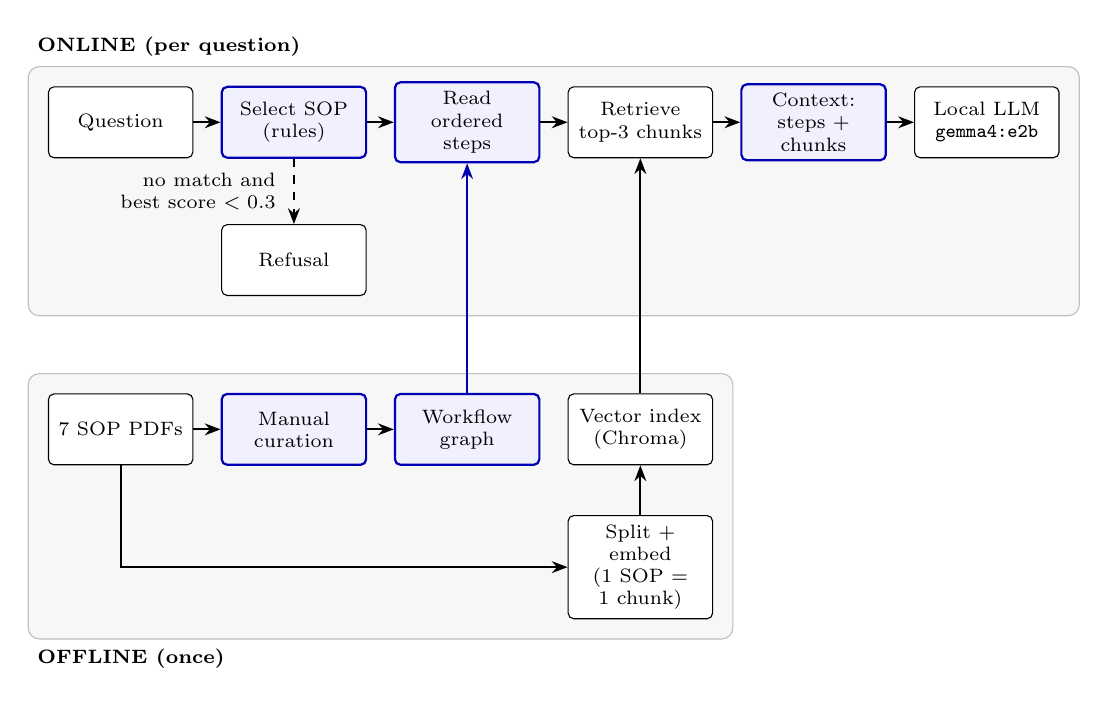
\begin{tikzpicture}[
  box/.style={draw, rounded corners=2pt, align=center, font=\scriptsize, minimum height=9mm, text width=16mm, fill=white},
  new/.style={box, draw=blue!70!black, fill=blue!6, thick},
  arr/.style={-{Stealth[length=2mm]}, thick},
  lane/.style={draw=gray!50, rounded corners=4pt, fill=gray!6, inner sep=2.5mm}
]
% Online row
\node[box] (q)    at (0,0)    {Question};
\node[new] (sel)  at (2.2,0)  {Select SOP\\(rules)};
\node[new] (read) at (4.4,0)  {Read ordered\\steps};
\node[box] (ret)  at (6.6,0)  {Retrieve\\top-3 chunks};
\node[new] (ctx)  at (8.8,0)  {Context:\\steps + chunks};
\node[box] (llm)  at (11.0,0) {Local LLM\\\texttt{gemma4:e2b}};
\node[box] (ref)  at (2.2,-1.75) {Refusal};
\draw[arr] (q) -- (sel);
\draw[arr] (sel) -- (read);
\draw[arr] (read) -- (ret);
\draw[arr] (ret) -- (ctx);
\draw[arr] (ctx) -- (llm);
\draw[arr, dashed] (sel) -- node[left, font=\scriptsize, align=right, xshift=-1mm]{no match and\\best score $<0.3$} (ref);
% Offline rows
\node[box] (pdf)    at (0,-3.9)   {7 SOP PDFs};
\node[new] (cur)    at (2.2,-3.9) {Manual\\curation};
\node[new] (graph)  at (4.4,-3.9) {Workflow\\graph};
\node[box] (chroma) at (6.6,-3.9) {Vector index\\(Chroma)};
\node[box] (split)  at (6.6,-5.65) {Split + embed\\(1 SOP = 1 chunk)};
\draw[arr] (pdf) -- (cur);
\draw[arr] (cur) -- (graph);
\draw[arr] (pdf.south) |- (split.west);
\draw[arr] (split) -- (chroma);
\draw[arr, blue!70!black] (graph) -- (read);
\draw[arr] (chroma) -- (ret);
\begin{scope}[on background layer]
\node[lane, fit=(q)(llm)(ref)] (on) {};
\node[lane, fit=(pdf)(split)(chroma)] (off) {};
\end{scope}
\node[font=\scriptsize\bfseries, anchor=south west] at (on.north west) {ONLINE (per question)};
\node[font=\scriptsize\bfseries, anchor=north west] at (off.south west) {OFFLINE (once)};
\end{tikzpicture}}
\caption{Architecture of Process-Aware Workflow GraphRAG. Highlighted nodes indicate components introduced: rule-based SOP selection and ordered workflow graph extraction. The underlying vector index, embedding model, prompt template, and generator are shared across evaluated systems.}
\label{fig:arch}
\end{figure}

\subsection{Workflow graph construction}
\label{sec:graph}
Each procedural document $p$ is represented as a directed graph $G_p = (V_p, E_p)$ implemented via NetworkX. The node set $V_p$ comprises three distinct classes:
\begin{enumerate}[leftmargin=*]
\item \textbf{Root Node ($v_{\text{root}}$):} Represents the complete procedure, storing the official title, administrative aliases (e.g., ``cuti kuliah'' for academic leave), and official maximum execution duration where specified.
\item \textbf{Step Nodes ($v_i$):} Encapsulates individual procedural steps $i \in \{1, \dots, n_p\}$. Each node stores: the primary performing actor; action description; required input documents; resulting deliverables; duration; and a verbatim textual quote from the source PDF.
\item \textbf{Actor Nodes ($v_{\text{actor}}$):} Represents distinct organizational roles or administrative offices shared across procedures.
\end{enumerate}

Edges $E_p$ capture three relationship types:
\begin{itemize}[leftmargin=*]
\item $\texttt{HAS\_STEP}(v_{\text{root}}, v_i)$: Links the procedure root to each constituent step.
\item $\texttt{NEXT\_STEP}(v_i, v_{i+1})$: Encodes chronological execution precedence between consecutive steps.
\item $\texttt{PERFORMS}(v_{\text{actor}}, v_i)$: Attributes operational execution of step $v_i$ to a specific actor node.
\end{itemize}

The workflow graph was constructed by hand from the 7 official PDFs, producing 7 root nodes, 44 step nodes, and 15 actor nodes connected by 125 directed edges. Steps were defined such that the primary actor corresponds to the operational performing entity (the grammatical subject of the procedural instruction), whereas consulted or secondary signatories are recorded within the action description. Automated verification scripts verified that every step quote matches the source text verbatim and that step counts align exactly with source PDFs. Figure~\ref{fig:graphs} contrasts this representation with the entity-graph baseline.

\begin{figure}[!htbp]
\centering
\resizebox{\textwidth}{!}{%
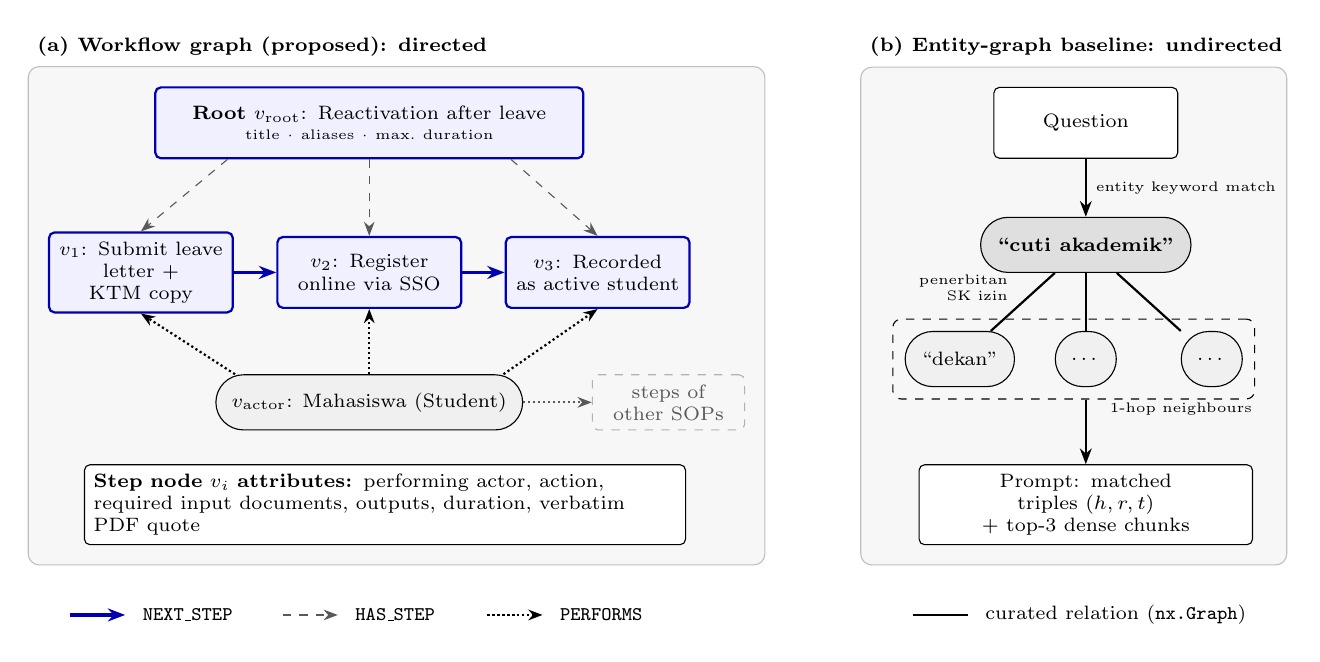
\begin{tikzpicture}[
  box/.style={execute at begin node={\hyphenpenalty=10000\exhyphenpenalty=10000}, draw, rounded corners=2pt, align=center, font=\scriptsize, minimum height=9mm, text width=21mm, fill=white},
  new/.style={box, draw=blue!70!black, fill=blue!6, thick},
  pill/.style={draw, rounded corners=3.5mm, align=center, font=\scriptsize, minimum height=7mm, inner xsep=2mm, fill=gray!12},
  ghost/.style={draw=gray!60, dashed, rounded corners=2pt, align=center, font=\scriptsize, text=gray!70!black, minimum height=7mm, text width=17mm},
  arr/.style={-{Stealth[length=2mm]}, thick},
  next/.style={-{Stealth[length=2.2mm]}, very thick, blue!70!black},
  has/.style={-{Stealth[length=1.8mm]}, gray!70!black, dashed},
  perf/.style={-{Stealth[length=1.8mm]}, densely dotted, thick},
  rel/.style={thick},
  lane/.style={draw=gray!50, rounded corners=4pt, fill=gray!6, inner sep=2.5mm}
]
% ===================== (a) Workflow graph (proposed) =====================
\node[new, text width=52mm] (root) at (2.9,0)
  {\textbf{Root} $v_{\text{root}}$: Reactivation after leave\\[-1pt]{\tiny title $\cdot$ aliases $\cdot$ max.\ duration}};
\node[new] (s1) at (0,-1.9)   {$v_1$: Submit leave\\letter + KTM copy};
\node[new] (s2) at (2.9,-1.9) {$v_2$: Register\\online via SSO};
\node[new] (s3) at (5.8,-1.9) {$v_3$: Recorded\\as active student};
\draw[has] (root.south) ++(-1.8,0) -- (s1.north);
\draw[has] (root.south) -- (s2.north);
\draw[has] (root.south) ++(1.8,0) -- (s3.north);
\draw[next] (s1) -- (s2);
\draw[next] (s2) -- (s3);
\node[pill] (act) at (2.9,-3.55) {$v_{\text{actor}}$: Mahasiswa (Student)};
\draw[perf] (act.north west) ++(0.25,0) -- (s1.south);
\draw[perf] (act.north) -- (s2.south);
\draw[perf] (act.north east) ++(-0.25,0) -- (s3.south);
\node[ghost] (oth) at (6.7,-3.55) {steps of\\other SOPs};
\draw[perf, gray!70!black] (act.east) -- (oth.west);
\node[draw, rounded corners=2pt, fill=white, font=\scriptsize, align=left, execute at begin node={\hyphenpenalty=10000}, text width=74mm] (attr) at (3.1,-4.85)
  {\textbf{Step node $v_i$ attributes:} performing actor, action, required input documents, outputs, duration, verbatim PDF quote};
% ===================== (b) Entity-graph baseline =====================
\node[box] (q) at (12.0,0) {Question};
\node[pill, fill=gray!25, font=\scriptsize\bfseries] (ent) at (12.0,-1.55) {``cuti akademik''};
\draw[arr] (q) -- node[right, font=\tiny]{entity keyword match} (ent);
\node[pill] (n1) at (10.4,-3.0)  {``dekan''};
\node[pill] (n2) at (12.0,-3.0) {\dots};
\node[pill] (n3) at (13.6,-3.0) {\dots};
\draw[rel] (ent) -- node[above left, pos=0.55, font=\tiny, align=right, inner sep=1pt, xshift=-1mm]{penerbitan\\SK izin} (n1);
\draw[rel] (ent) -- (n2);
\draw[rel] (ent) -- (n3);
\node[draw, dashed, rounded corners=3pt, fit=(n1)(n3), inner sep=1.5mm,
      label={[font=\tiny, anchor=north east, inner sep=1pt]south east:1-hop neighbours}] (hop) {};
\node[box, text width=40mm] (pr) at (12.0,-4.85) {Prompt: matched triples $(h,r,t)$\\+ top-3 dense chunks};
\draw[arr] (pr.north |- hop.south) -- (pr.north);
% ===================== Panels and legend =====================
\begin{scope}[on background layer]
\node[lane, fit=(root)(s1)(s3)(act)(oth)(attr)] (pa) {};
\node[lane, fit=(q)(n1)(n3)(hop)(pr), inner xsep=4mm] (pb) {};
\end{scope}
\node[font=\scriptsize\bfseries, anchor=south west] at (pa.north west) {(a) Workflow graph (proposed): directed};
\node[font=\scriptsize\bfseries, anchor=south west] at (pb.north west) {(b) Entity-graph baseline: undirected};
\begin{scope}[yshift=-6.25cm, font=\scriptsize]
\draw[next] (-0.9,0) -- (-0.2,0); \node[anchor=west] at (-0.1,0) {\texttt{NEXT\_STEP}};
\draw[has]  (1.8,0) -- (2.5,0);   \node[anchor=west] at (2.6,0)  {\texttt{HAS\_STEP}};
\draw[perf] (4.4,0) -- (5.1,0);   \node[anchor=west] at (5.2,0)  {\texttt{PERFORMS}};
\draw[rel]  (9.8,0) -- (10.5,0);   \node[anchor=west] at (10.6,0)  {curated relation (\texttt{nx.Graph})};
\end{scope}
\end{tikzpicture}}
\caption{Graph representations compared in this study. (a) The proposed workflow graph, shown for the \emph{Reactivation after leave} SOP: the root node links to each step via \texttt{HAS\_STEP}, \texttt{NEXT\_STEP} edges encode execution order, and \texttt{PERFORMS} edges attribute each step to an actor node shared across procedures. The full graph contains 7 root, 44 step, and 15 actor nodes connected by 125 directed edges. (b) The custom entity-graph baseline: question entities are matched against 17 curated relational triples in an undirected graph, and the 1-hop triples are prepended to the top-3 dense chunks.}
\label{fig:graphs}
\end{figure}

\subsection{Rule-based SOP selection}
Given user question $q$, the system identifies the target procedure $p^\ast$ using a transparent heuristic scoring function:
\begin{equation}
s(q,p) = 15\,\mathbb{1}[\textit{title}_p \subset q] + \sum_{a \in \textit{aliases}_p} g(q,a) + \sum_{v \in \textit{steps}_p} h(q,v),
\label{eq:score}
\end{equation}
where $g(q,a) = 8$ if alias $a$ occurs as an exact substring in $q$, or 2 per constituent word ($|w| > 2$); and $h(q,v) = 1$ if $q$ contains an explicit procedural cue (Indonesian keywords for ``how'', ``procedure'', ``requirements'', ``flow'', or ``documents'') and shares a content word ($|w| > 4$) with the step action description.

The procedure with the maximum score is selected if $s(q,p^\ast) \geq 3$. A deterministic priority rule maps questions simultaneously containing keywords for ``active'' and ``leave'' to \emph{Reactivation after leave}, resolving potential confusion between the two procedures. Matching is case-insensitive. While rule-based matching is deterministic and inspectable, it is tailored to this 7-SOP collection.

\subsection{Context construction and supporting retrieval}
When procedure $p^\ast$ is selected, its step nodes are extracted via a topological traversal along $\texttt{NEXT\_STEP}$ edges. The steps are serialized into an ordered textual context block specifying step index, performing actor, action, required documents, outputs, and duration (Figure~\ref{fig:context}).

\begin{figure}[!htbp]
\centering
\small
\fbox{\begin{minipage}{0.92\textwidth}
\textbf{OFFICIAL WORKFLOW: REACTIVATION AFTER LEAVE (AKTIF KEMBALI)}\\
Maximum processing duration: Not specified in document\\[2pt]
\textbf{Step 1.} Actor: Mahasiswa (Student)\\
\hspace*{1em}Action: Submit academic leave permit letter from prior semester and student card copy to Head of Study Programme and Academic Sub-division.\\
\hspace*{1em}Required Documents: Academic leave permit letter, Student card (KTM) copy\\
\hspace*{1em}Duration: $\pm$5 minutes\\[2pt]
\textbf{Step 2.} Actor: Mahasiswa (Student)\\
\hspace*{1em}Action: Register online for reactivation through university Single Sign-On (SSO) portal.\\
\hspace*{1em}\dots\\[2pt]
\textbf{Step 3.} Actor: Mahasiswa (Student)\\
\hspace*{1em}Action: Registered as active course participant in academic database.\\
\hspace*{1em}\dots\\[2pt]
\textbf{Supporting Documents:} \textit{[Top-3 dense chunks retrieved from vector store]}
\end{minipage}}
\caption{Illustrative context block produced for reactivation inquiry (translated from Indonesian). Each step explicitly details performing actor, action, and required documentation.}
\label{fig:context}
\end{figure}

To provide access to supplementary document details (such as administrative notes and URLs), the query is expanded by concatenating $q$ with the SOP title and actions from its first three steps. Dense retrieval queries the shared Chroma vector index using the expanded query, retrieving $k=3$ supporting chunks that are appended after the workflow block. Because each chunk in the vector index corresponds to one SOP, these supporting chunks may contain text from other SOPs, which we analyze in Section~\ref{sec:discussion}.

\subsection{Generation and refusal mechanism}
Context and question are injected into a standard prompt template instructing the model to respond in Indonesian, adhere strictly to provided context facts, and abstain if evidence is insufficient. Inference is executed locally using \texttt{gemma4:e2b} via Ollama.

Refusal operates through a combination of deterministic pre-generation filtering and model-generated abstention. Deterministic refusal triggers before generator invocation if: (1) no SOP satisfies selection ($s(q,p^\ast) < 3$); and (2) maximum cosine similarity of $q$ against retrieved vector chunks is below threshold $\tau = 0.3$. If an SOP is selected, the query proceeds to the generator, which can still produce a refusal response if the provided context lacks the requested facts. Algorithm~\ref{alg:workflow} details the execution pipeline.

\begin{algorithm}[!htbp]
\caption{Execution pipeline of Process-Aware Workflow GraphRAG}
\label{alg:workflow}
\begin{algorithmic}[1]
\REQUIRE Question $q$, workflow graph $G$, vector index $I$, threshold $\tau = 0.3$, retrieval depth $k=3$
\STATE $p^\ast \leftarrow \arg\max_p s(q,p)$ \COMMENT{Evaluate selection via Eq.~\eqref{eq:score}}
\IF{$s(q,p^\ast) < 3$}
  \STATE $p^\ast \leftarrow \text{none}$
\ENDIF
\IF{$p^\ast \neq \text{none}$}
  \STATE $W \leftarrow$ serialized ordered step sequence of $p^\ast$ from $G$
  \STATE $q' \leftarrow q \,\|\, \textit{title}_{p^\ast} \,\|\, \textit{actions}_{1:3}(p^\ast)$ \COMMENT{Query expansion}
\ELSE
  \STATE $W \leftarrow \emptyset$
  \STATE $q' \leftarrow q$ \COMMENT{Retain unexpanded query}
\ENDIF
\STATE $C \leftarrow \textsc{RetrieveTopK}(I, q', k)$
\STATE $b \leftarrow \max_{c \in C} \textsc{CosineSimilarity}(q, c)$
\IF{$p^\ast = \text{none}$ \AND $b < \tau$}
  \RETURN Refusal response (``Information not available in official SOPs'')
\ENDIF
\RETURN $\textsc{GenerateLocalLLM}(\textsc{PromptTemplate}(W \,\|\, C, q))$
\end{algorithmic}
\end{algorithm}

\subsection{Selection-matched text ablation design}
\label{sec:ablation-oracle}
A central methodological question is whether observed performance gains stem from explicit workflow graph structuring or from procedure selection. To isolate these factors, we implement \emph{Selection-Matched Text RAG} (designated in experimental benchmark logs as \emph{SOP-Oracle RAG}).

This ablation shares the identical SOP selection rule (Eq.~\eqref{eq:score}) and query-expanded supporting chunk retrieval as Workflow GraphRAG. However, instead of serializing the workflow graph $W$, it retrieves the raw, unedited text chunk of the selected SOP $p^\ast$ from the document store. Thus, both systems receive the identical procedure and supporting chunks, differing solely in representation: structured workflow block vs.\ original unstructured prose. Figure~\ref{fig:prompt} shows the resulting context supplied to each main comparison system.

\begin{figure}[!htbp]
\centering
\resizebox{\textwidth}{!}{%
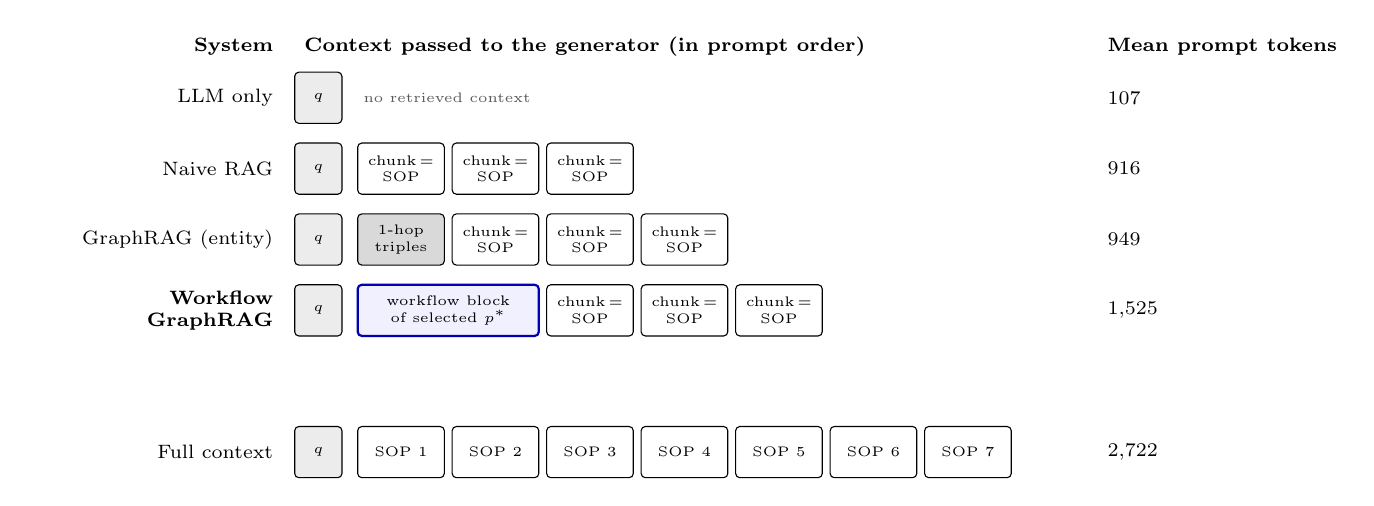
\begin{tikzpicture}[
  lab/.style={anchor=east, font=\scriptsize, align=right, text width=30mm},
  blk/.style={draw, rounded corners=1.5pt, font=\tiny, align=center, minimum height=6.5mm, minimum width=11mm, inner sep=1pt, fill=white},
  q/.style={blk, minimum width=6mm, fill=gray!15},
  sel/.style={blk, draw=blue!70!black, fill=blue!6, thick, minimum width=23mm},
  trip/.style={blk, fill=gray!30, minimum width=11mm},
  tok/.style={anchor=west, font=\scriptsize}
]
\def\dx{1.2}
% header
\node[font=\scriptsize\bfseries, anchor=east] at (-0.15,0.65) {System};
\node[font=\scriptsize\bfseries, anchor=west] at (0,0.65) {Context passed to the generator (in prompt order)};
\node[font=\scriptsize\bfseries, anchor=west] at (10.2,0.65) {Mean prompt tokens};
% LLM only
\node[lab] at (-0.15,0) {LLM only};
\node[q] at (0.3,0) {$q$};
\node[font=\tiny, anchor=west, text=gray!70!black] at (0.75,0) {no retrieved context};
\node[tok] at (10.2,0) {107};
% Naive
\node[lab] at (-0.15,-0.9) {Naive RAG};
\node[q] at (0.3,-0.9) {$q$};
\foreach \i in {1,2,3} \node[blk] at (0.75+\i*\dx-0.6,-0.9) {chunk\,=\\SOP};
\node[tok] at (10.2,-0.9) {916};
% Entity graph
\node[lab] at (-0.15,-1.8) {GraphRAG (entity)};
\node[q] at (0.3,-1.8) {$q$};
\node[trip] at (1.35,-1.8) {1-hop\\triples};
\foreach \i in {1,2,3} \node[blk] at (1.95+\i*\dx-0.6,-1.8) {chunk\,=\\SOP};
\node[tok] at (10.2,-1.8) {949};
% Workflow
\node[lab] at (-0.15,-2.7) {\textbf{Workflow GraphRAG}};
\node[q] at (0.3,-2.7) {$q$};
\node[sel] at (1.95,-2.7) {workflow block\\of selected $p^\ast$};
\foreach \i in {1,2,3} \node[blk] at (3.15+\i*\dx-0.6,-2.7) {chunk\,=\\SOP};
\node[tok] at (10.2,-2.7) {1,525};
% Selection-matched
\ifshoworacle
\node[lab] at (-0.15,-3.6) {Selection-Matched Text (ablation)};
\node[q] at (0.3,-3.6) {$q$};
\node[sel, thin, fill=blue!3] at (1.95,-3.6) {raw PDF text\\of selected $p^\ast$};
\foreach \i in {1,2,3} \node[blk] at (3.15+\i*\dx-0.6,-3.6) {chunk\,=\\SOP};
\node[tok] at (10.2,-3.6) {1,479};
\fi
% Full context
\node[lab] at (-0.15,-4.5) {Full context};
\node[q] at (0.3,-4.5) {$q$};
\foreach \i in {1,...,7} \node[blk] at (0.75+\i*\dx-0.6,-4.5) {SOP \i};
\node[tok] at (10.2,-4.5) {2,722};
\end{tikzpicture}}
\caption{Context supplied to the generator by the main comparison systems. Because every SOP fits in one 1,700-character chunk, each retrieved chunk is a complete SOP, so top-3 retrieval always places three procedures in the prompt (Section~3.3). Workflow GraphRAG and the selection-matched ablation share the selection rule and the same top-3 supporting chunks, which may come from unselected SOPs, and differ only in how the selected procedure $p^\ast$ is represented. Token counts are means over all 40 questions and include the shared prompt template and question.}
\label{fig:prompt}
\end{figure}

%% ===================================================================
\section{Experimental setup}
\label{sec:setup}

\subsection{Evaluated systems}
\label{sec:systems}
We evaluate 10 system configurations grouped into three functional categories (Table~\ref{tab:systems}):
\begin{enumerate}[leftmargin=*]
\item \textbf{Main Comparison Systems:}
  \begin{itemize}
  \item \emph{Naive RAG:} Standard baseline retrieving top-3 dense chunks. Refuses if top similarity $< 0.3$.
  \item \emph{Custom Entity-Graph GraphRAG:} Baseline matching question entities against a hand-curated undirected graph of 17 relational triples (e.g., procedure linked to responsible office or required document), expanding to 1-hop neighbors, appending relation triples to prompt, and retrieving top-3 chunks.
  \item \emph{Workflow GraphRAG (Proposed):} Full architecture combining rule-based SOP selection, ordered workflow graph serialization, and supporting chunk retrieval.
  \item \emph{Selection-Matched Text RAG (Ablation):} Identical selection and supporting chunks as Workflow GraphRAG, supplying raw SOP text in place of graph serialization.
  \end{itemize}
\item \textbf{Supplementary RAG Baselines:}
  \begin{itemize}
  \item \emph{Hybrid RAG:} Dense top-5 and BM25 top-5 retrieval merged via Reciprocal Rank Fusion ($k_{\text{rrf}}=60$), retaining top-3 chunks.
  \item \emph{Agentic RAG:} Multi-turn ReAct reasoning loop allowing up to 3 iterative search actions prior to generation.
  \item \emph{Corrective RAG (CRAG):} Evaluates retrieval confidence; scores $\geq 0.55$ proceed directly, $0.35$--$0.55$ trigger LLM query rewriting, $< 0.35$ are refused.
  \item \emph{Multimodal-Layout RAG:} Dense retrieval incorporating structural document cues (table and section tags) extracted during ingestion.
  \end{itemize}
\item \textbf{Reference Systems:}
  \begin{itemize}
  \item \emph{LLM Only:} Parametric generation without retrieval, establishing base generator knowledge.
  \item \emph{Full-Context Prompting:} Supplies all 7 SOP documents ($\approx$1,100 words) in the prompt, representing an upper bound on available evidence without retrieval filtering.
  \end{itemize}
\end{enumerate}

\begin{table}[!htbp]
\centering
\caption{System configurations evaluated across 10 architectures. All systems share identical embedding models, chunking parameters (1,700/100 characters), vector stores, generator, and prompt templates.}
\label{tab:systems}
\small
\begin{tabularx}{\textwidth}{>{\raggedright\arraybackslash}p{3.5cm} >{\raggedright\arraybackslash}X}
\toprule
System Configuration & Context Construction and Retrieval Mechanism \\
\midrule
\multicolumn{2}{l}{\textit{Main Comparison and Ablation}} \\
Naive RAG & Top-3 dense chunks by cosine similarity; refuses if best similarity $< 0.3$. \\
GraphRAG (custom entity graph) & 1-hop expansion over 17 curated relational triples; matched triples prepended to top-3 dense chunks. \\
\textbf{Workflow GraphRAG (proposed)} & Ordered workflow steps from directed graph with explicit actors and inputs, followed by top-3 supporting chunks. \\
\textit{Selection-Matched Text RAG (SOP-Oracle ablation)} & Identical rule-based selection, providing selected raw SOP text in place of workflow block, followed by top-3 supporting chunks. \\
\midrule
\multicolumn{2}{l}{\textit{Supplementary RAG Baselines}} \\
Hybrid RAG & Reciprocal rank fusion of top-5 dense and top-5 BM25 chunks ($k_{\text{rrf}}=60$); top-3 retained. \\
Agentic RAG & ReAct loop executing up to 3 iterative search queries directed by generator. \\
Corrective RAG (CRAG) & Retrieval grading: $\geq 0.55$ retained, $0.35$--$0.55$ query rewritten, $< 0.35$ refused. \\
Multimodal-Layout RAG & Top-3 dense chunks augmented with structural document layout tags. \\
\midrule
\multicolumn{2}{l}{\textit{Reference Baselines}} \\
LLM Only & Zero-shot generation without retrieved context. \\
Full-Context Prompting & All 7 SOP documents provided directly in generator prompt ($\approx$1,100 words). \\
\bottomrule
\end{tabularx}
\end{table}

\subsection{Custom entity-graph baseline scope and validity threat}
We explicitly state that the entity-graph GraphRAG baseline is an author-developed implementation consisting of 17 curated relational triples. It is not an official deployment of Microsoft GraphRAG \cite{edge2024graphrag}, LightRAG \cite{guo2024lightrag}, or HippoRAG \cite{gutierrez2024hipporag}. Because the baseline was constructed by the authors, it represents an empirical point of comparison for basic entity-triple augmentation rather than an exhaustive evaluation of published GraphRAG frameworks. The complete set of triples is listed in Appendix~\ref{app:triples}. We treat this as an explicit validity constraint in Section~\ref{sec:discussion}.

\subsection{Shared infrastructure and experimental controls}
All retrieval systems share identical underlying infrastructure:
\begin{itemize}[leftmargin=*]
\item \textbf{Embedding Model:} \texttt{all-indo-e5-small-v4} \cite{lazarusnlp_e5}, an Indonesian sentence embedder (384 dimensions) fine-tuned on 50 procedural question-answer pairs using Multiple Negatives Ranking (MNR) loss \cite{henderson2017mnr}. An ablation evaluates the non-fine-tuned base model.
\item \textbf{Vector Store:} Chroma vector database storing 7 chunks (1,700 character window, 100 character overlap).
\item \textbf{Generator:} \texttt{gemma4:e2b} (5.1B total parameters, Q4\_K\_M quantization) served locally via Ollama 0.35.1 at temperature 0, seed 42, following one warm-up inference.
\item \textbf{Hardware and Invocation Logging:} Apple M5 workstation (10 CPU cores, 24~GB unified memory) running macOS 26.6.2 on AC power. Every generator call records prompt tokens, completion tokens, and latency via unified logging wrappers. The mean number of generator invocations per query reflects deterministic pre-generation refusal: systems that filter out low-similarity queries prior to inference average fewer than 1.00 calls across the benchmark.
\end{itemize}

\subsection{Evaluation benchmark}
We developed a held-out benchmark of 40 questions drafted from the source SOPs (Table~\ref{tab:bench}). The benchmark items were not generated by any evaluated system, and a lexical overlap audit confirmed no question shares ROUGE-L $\geq 0.5$ with the fine-tuning training pairs. One example question per category is given in Appendix~\ref{app:examples}.

\begin{table}[!htbp]
\centering
\caption{Composition of the 40-question held-out institutional benchmark.}
\label{tab:bench}
\small
\setlength{\tabcolsep}{4pt}
\begin{tabularx}{\textwidth}{lr>{\raggedright\arraybackslash}X}
\toprule
Category & $n$ & Operational Target \\
\midrule
Procedural & 11 & Complete step sequence, chronological order, and actors (7 formal, 4 colloquial). \\
Actor attribution & 7 & Identification of verifying, signing, or receiving officials. \\
Document requirements & 7 & Identification of mandatory forms, attachments, and outputs. \\
Time and location & 7 & Stated execution durations, service desks, and IT portals. \\
Cross-SOP discrimination & 3 & Differentiating easily confused procedures (evaluating E3). \\
Unanswerable / Refusal & 5 & Inquiries concerning out-of-scope administrative rules. \\
\midrule
Total & 40 & \\
\bottomrule
\end{tabularx}
\end{table}

The benchmark contains 35 answerable questions (comprising 32 single-SOP questions across procedural, actor, document, and time categories, plus 3 cross-SOP questions) and 5 unanswerable questions. Each answerable item defines a reference answer and required key facts. Each procedural item additionally specifies a gold sequence of execution steps, associated actors, and matching keyword groups. All items were verified against official PDFs by the first author.

\subsection{Evaluation metrics}
Evaluation metrics are computed deterministically without reliance on LLM judges:
\begin{itemize}[leftmargin=*]
\item \textbf{Key-Fact Recall (KFR):} Proportion of required reference facts detected in the generated response, evaluated across the 35 answerable questions.
\item \textbf{ROUGE-1, ROUGE-2, ROUGE-L:} Standard n-gram and longest common subsequence overlap against reference answers \cite{lin2004rouge}.
\item \textbf{Step Coverage:} For procedural questions ($n=11$), proportion of gold steps $S$ detected in the generated response ($|D|/|S|$), where detection requires matching at least two keyword groups.
\item \textbf{Topological Inversion Rate (TIR):} Proportion of detected step pairs $(v_i, v_j)$ with $i < j$ that appear in reversed order in the response:
\begin{equation}
\text{TIR} = \frac{\bigl|\{(v_i,v_j) \in D^2 : i<j,\ \textit{pos}(v_i) > \textit{pos}(v_j)\}\bigr|}{\bigl|\{(v_i,v_j) \in D^2 : i<j,\ \textit{pos}(v_i) \neq \textit{pos}(v_j)\}\bigr|}.
\end{equation}
TIR is conditional on detecting at least two comparable steps.
\item \textbf{Actor Mismatch Rate (AMR):} Proportion of detected steps attributed to an incorrect official among steps where an actor is explicitly named:
\begin{equation}
\text{AMR} = \frac{\textit{mismatch}}{\textit{correct} + \textit{mismatch}}.
\end{equation}
AMR is conditional on step detection and explicit actor naming.
\item \textbf{Refusal Accuracy and False Refusal Rate:} Refusal accuracy is the proportion of the 5 unanswerable questions correctly refused. False refusal rate is the proportion of the 35 answerable questions incorrectly refused.
\item \textbf{Resource Costs:} Prompt tokens, completion tokens, LLM invocations, and elapsed latency per question, averaged across all 40 benchmark items.
\end{itemize}

\subsection{Manual audit of deterministic step scorer}
\label{sec:audit}
Because step detection, TIR, and AMR depend on keyword matching, we audited the deterministic scorer. A sample of 60 step-alignment rows was drawn across Naive RAG, GraphRAG, and Workflow GraphRAG (stratified, seed 42) and evaluated manually by the first author against full response texts (Table~\ref{tab:audit}).

\begin{table}[!htbp]
\centering
\caption{Manual audit of deterministic step-alignment scorer across 60 sampled rows (Naive RAG, GraphRAG, and Workflow GraphRAG).}
\label{tab:audit}
\small
\begin{tabular}{lcc}
\toprule
Measure & Agreement / $\kappa$ & Labelled \\
\midrule
Step detected & 0.983 / 0.955 & 60/60 \\
Actor status & 0.933 / 0.835 & 60/60 \\
\bottomrule
\end{tabular}

\end{table}

The manual audit demonstrated 0.983 agreement ($\kappa=0.955$) on step detection and 0.933 agreement ($\kappa=0.835$) on actor attribution across the 60 sampled rows. The single step detection discrepancy occurred on GraphRAG for late tuition payment (UKT-P1, step 5), where the model formatted actor and action on separate markdown bullet lines (``\textbf{Pelaku:} Wakil Dekan Sumber Daya'' followed by ``\textbf{Tindakan:} Memproses\dots''). Because the scorer segments text line-by-line and requires two keyword groups per line, it recorded a non-detection despite both elements being present. Crucially, the manual audit confirmed zero genuine actor attribution errors across the 60 sampled rows ($\text{AMR} = 0.000$). We note that this audit validates scorer fidelity for the audited sample, but does not imply zero actor errors across all uninspected generated texts.

\subsection{Secondary LLM-as-a-judge metrics}
As a supplementary check, Ragas faithfulness and answer relevancy \cite{es2024ragas} were computed using an independent judge model (\texttt{llama3.1:8b}) \cite{zheng2023judging}. Faithfulness evaluates claims against provided context (including workflow blocks). Due to occasional JSON parsing failures in the judge output (yielding valid scores for 35/40 questions in Workflow GraphRAG and 26--27/40 in baselines), Ragas metrics are treated strictly as secondary corroboration.

\subsection{Statistical testing methodology}
To account for benchmark sample size ($n=40$), all metrics report sample means with 95\% bootstrap confidence intervals (10,000 resamples) \cite{efron1993bootstrap}. Comparisons between Workflow GraphRAG and baselines utilize two-sided paired Wilcoxon signed-rank tests \cite{wilcoxon1945}. Holm-Bonferroni correction \cite{holm1979} is applied within distinct hypothesis testing families (separately for the family of comparisons against Naive RAG and against GraphRAG).

We emphasize that bootstrap confidence intervals and Holm-adjusted hypothesis tests operate under distinct multiplicity assumptions: a confidence interval for a single pairwise difference may exclude zero while the corresponding family-wise adjusted $p$-value exceeds $\alpha = 0.05$. We report both transparently and avoid describing non-significant results as established equivalence.

%% ===================================================================
\section{Experimental results}
\label{sec:results}

Empirical evaluations are derived from the execution run on all \nVerified{} verified benchmark items (\url{results/full_v3_20261008/}, branch \url{exp/full-run-v1}).

\subsection{Procedural answer quality and order preservation (RQ1)}
Table~\ref{tab:results} reports performance across all 10 evaluated systems. Workflow GraphRAG, Selection-Matched Text RAG, and Full-Context Prompting achieve top-tier performance on key-fact recall: 0.955 [0.917, 0.990], 0.962 [0.914, 1.000], and 0.962 [0.914, 1.000], respectively. In contrast, Naive RAG achieves 0.712 [0.571, 0.840] and custom entity-graph GraphRAG achieves 0.698 [0.560, 0.829]. Workflow GraphRAG attains 1.000 [1.000, 1.000] step coverage on procedural questions, compared to 0.727 for Naive RAG and 0.687 for GraphRAG.

\begin{table}[!htbp]
\centering
\caption{Summary of evaluation results across ten system configurations. Key-fact recall (KFR) and false refusal rate are evaluated on 35 answerable questions; procedural metrics (Coverage, TIR, AMR) on 11 procedural questions; refusal accuracy on 5 unanswerable questions; and prompt tokens on all 40 questions. Values are point estimates; full bootstrap 95\% confidence intervals are reported in Appendix~\ref{app:full-results}. TIR: Topological Inversion Rate; AMR: Actor Mismatch Rate.}
\label{tab:results}
\small
\setlength{\tabcolsep}{2pt}
\resizebox{\textwidth}{!}{%
\begin{tabular}{lccccccc}
\toprule
System & KFR $\uparrow$ & Coverage $\uparrow$ & TIR $\downarrow$ & AMR $\downarrow$ & Refusal acc. $\uparrow$ & False ref. $\downarrow$ & Prompt tok. \\
\midrule
Naive RAG & 0.712 & 0.727 & 0.000 & 0.000 & 0.600 & 0.000 & 916 \\
GraphRAG (entity) & 0.698 & 0.687 & 0.083 & 0.000 & 0.600 & 0.000 & 949 \\
\textbf{Workflow GraphRAG} & 0.955 & 1.000 & 0.000 & 0.000 & 1.000 & 0.000 & 1525 \\
\textit{Selection-Matched Text RAG (ablation)} & 0.962 & 0.975 & 0.000 & 0.000 & 1.000 & 0.000 & 1479 \\
\midrule
Hybrid RAG & 0.683 & 0.712 & 0.000 & 0.000 & 0.600 & 0.000 & 882 \\
Agentic RAG & 0.712 & 0.702 & 0.000 & 0.000 & 0.600 & 0.000 & 1815 \\
Corrective RAG & 0.569 & 0.636 & 0.000 & 0.000 & 1.000 & 0.371 & 725 \\
Multimodal-layout RAG & 0.702 & 0.702 & 0.000 & 0.000 & 0.600 & 0.000 & 994 \\
\midrule
LLM only & 0.113 & 0.105 & 0.333 & 0.444 & 0.000 & 0.000 & 107 \\
Full context & 0.962 & 0.944 & 0.027 & 0.000 & 1.000 & 0.000 & 2722 \\
\bottomrule
\end{tabular}
}
\end{table}

Statistical testing indicates that Workflow GraphRAG demonstrates a statistically significant improvement over custom entity-graph GraphRAG in key-fact recall ($+0.257$ [0.133, 0.395], Holm-adjusted $p=0.034$) and ROUGE-L ($+0.077$ [0.031, 0.127], Holm-adjusted $p=0.038$), while step coverage differences are not statistically significant after adjustment ($p=0.438$).

When compared against Naive RAG, Workflow GraphRAG demonstrates an absolute improvement of $+0.243$ [0.114, 0.381] in key-fact recall. However, under Holm adjustment across the metric family, the difference yields $p = 0.053$. Because $p > 0.05$, we report this comparison as not reaching formal statistical significance at $\alpha = 0.05$. The unadjusted bootstrap confidence interval excludes zero, indicating a consistent empirical direction, but the sample size ($n=40$) limits conclusive statistical separation under family-wise error control.

Topological inversion rates (TIR) and actor mismatch rates (AMR) are detailed in Table~\ref{tab:results}. For steps actually detected, Workflow GraphRAG, Naive RAG, Selection-Matched Text RAG, and the supplementary RAG baselines achieved an observed TIR of 0.000, whereas the custom entity-graph baseline and full-context prompting exhibited non-zero inversion rates of 0.083 [0.000, 0.250] and 0.027 [0.000, 0.082], respectively (with the LLM-only reference at 0.333 [0.000, 0.667]). In actor attribution, all retrieval-augmented configurations achieved an observed AMR of 0.000 on detected steps where an actor was explicitly named, while LLM-only exhibited 0.444. These values must be interpreted jointly with step coverage: low inversion rates reflect that when steps are detected, they appear in order, but the primary performance separation among systems centers on procedural completeness and factual recall rather than reordering of generated steps.

Categorical breakdowns (Table~\ref{tab:percat}) indicate that Workflow GraphRAG achieves strong factual recall across procedural inquiries (1.000 vs.\ 0.727 for baselines) and cross-SOP inquiries (0.889 vs.\ 0.611). In cross-SOP questions requiring identification of signatories across distinct procedures, Workflow GraphRAG's step output fields enable unambiguous attribution, mitigating error E3.

\begin{table}[!htbp]
\centering
\caption{Key-fact recall by question category for the primary comparison systems on \nVerified{} verified questions. Procedural category also includes step coverage.}
\label{tab:percat}
\small
\setlength{\tabcolsep}{4pt}
\resizebox{\textwidth}{!}{%
% Key-fact recall per category (procedural column also has step coverage), for the three main systems
\begin{tabular}{lccccc}
\toprule
System & Procedural (KFR/Cov.) & Actor & Documents & Time/location & Cross-SOP \\
\midrule
Naive RAG & 0.727 / 0.727 & 0.857 & 0.619 & 0.679 & 0.611 \\
GraphRAG (entity) & 0.727 / 0.687 & 0.786 & 0.619 & 0.679 & 0.611 \\
\textbf{Workflow GraphRAG} & 1.000 / 1.000 & 0.952 & 0.905 & 0.964 & 0.889 \\
\bottomrule
\end{tabular}
}
\end{table}

\subsection{Selection versus structuring ablation (RQ2)}
\label{sec:ablation-results}
The comparison between Workflow GraphRAG (0.955 KFR) and Selection-Matched Text RAG (0.962 KFR; Table~\ref{tab:results}) addresses RQ2. The two systems share the identical SOP selection mechanism (Eq.~\eqref{eq:score}) and top-3 supporting chunk retrieval, differing only in whether the primary procedure is supplied as a structured graph block or as raw PDF text.

A paired Wilcoxon signed-rank test on answerable questions ($n=35$) yields a paired mean difference of $-0.007$ [$-0.036$, $0.021$] with $p = 0.59$. Factual scores differ on only 3 of 35 questions. This empirical test does not detect a statistically significant difference between graph-structured context and selection-matched text context. We emphasize that $p=0.59$ does not prove equivalence between the two representations; rather, the data provide no evidence that explicit graph serialization confers an incremental factual accuracy advantage over supplying the selected procedure's raw text on this benchmark.
Figure~\ref{fig:forest} places this comparison alongside the comparisons against chunk retrieval.

\begin{figure}[!htbp]
\centering
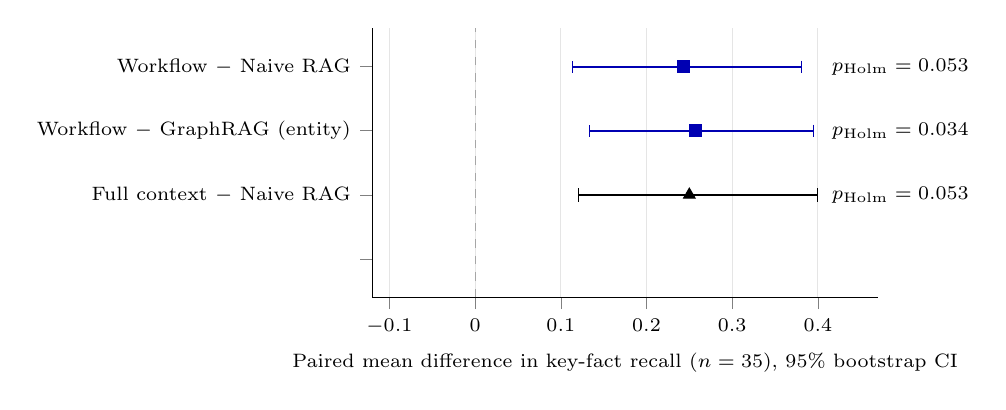
\begin{tikzpicture}
\begin{axis}[
  width=0.66\textwidth, height=5.0cm,
  xmin=-0.12, xmax=0.47, ymin=0.4, ymax=4.6,
  ytick={1,2,3,4},
  yticklabels={
    \ifshoworacle Workflow $-$ Selection-Matched\else\fi,
    Full context $-$ Naive RAG,
    Workflow $-$ GraphRAG (entity),
    Workflow $-$ Naive RAG},
  yticklabel style={font=\scriptsize, align=right},
  xticklabel style={font=\scriptsize, /pgf/number format/fixed, /pgf/number format/precision=2},
  xlabel={Paired mean difference in key-fact recall ($n=35$), 95\% bootstrap CI},
  xlabel style={font=\scriptsize},
  axis lines*=left, tick align=outside, clip=false,
  xmajorgrids, grid style={gray!20},
]
\draw[gray!70, dashed] (axis cs:0,0.4) -- (axis cs:0,4.6);
% Workflow - Naive: 0.243 [0.114, 0.381], Holm p = 0.053
\addplot[blue!70!black, only marks, mark=square*, mark size=2.2pt, error bars/.cd, x dir=both, x explicit, error bar style={thick}]
  coordinates {(0.243,4) += (0.138,0) -= (0.129,0)};
% Workflow - GraphRAG: 0.257 [0.133, 0.395], Holm p = 0.034
\addplot[blue!70!black, only marks, mark=square*, mark size=2.2pt, error bars/.cd, x dir=both, x explicit, error bar style={thick}]
  coordinates {(0.257,3) += (0.138,0) -= (0.124,0)};
% Full context - Naive: 0.250 [0.121, 0.400], Holm p = 0.053
\addplot[black, only marks, mark=triangle*, mark size=2.4pt, error bars/.cd, x dir=both, x explicit, error bar style={thick}]
  coordinates {(0.250,2) += (0.150,0) -= (0.129,0)};
\ifshoworacle
% Workflow - Selection-Matched: -0.007 [-0.036, 0.021], Wilcoxon p = 0.59 (paper text; not in repository)
\addplot[blue!70!black, only marks, mark=square, mark size=2.2pt, error bars/.cd, x dir=both, x explicit, error bar style={thick}]
  coordinates {(-0.007,1) += (0.028,0) -= (0.029,0)};
\node[font=\scriptsize, anchor=west] at (axis cs:0.405,1) {$p=0.59$};
\fi
\node[font=\scriptsize, anchor=west] at (axis cs:0.405,4) {$p_{\mathrm{Holm}}=0.053$};
\node[font=\scriptsize, anchor=west] at (axis cs:0.405,3) {$p_{\mathrm{Holm}}=0.034$};
\node[font=\scriptsize, anchor=west] at (axis cs:0.405,2) {$p_{\mathrm{Holm}}=0.053$};
\end{axis}
\end{tikzpicture}
\caption{Paired differences in key-fact recall on the 35 answerable questions, with 95\% bootstrap confidence intervals and two-sided Wilcoxon signed-rank $p$-values (Holm-adjusted within each reference family). Gains over chunk retrieval appear for both Workflow GraphRAG and full-context prompting, whereas the selection-matched comparison, which holds procedure selection fixed, is centred near zero.}
\label{fig:forest}
\end{figure}

The apparent difference in step coverage (1.000 for Workflow GraphRAG vs.\ 0.975 for Selection-Matched Text RAG) traces to a single procedural item (UKT-P1). As identified in Section~\ref{sec:audit}, the ablation system formatted actor and action on distinct markdown lines, preventing the line-based deterministic scorer from registering step co-occurrence despite all 11 steps being present in the generated text.

Regarding selection performance, exactly 36 items in the benchmark assign a single procedure in their metadata (32 answerable single-SOP questions and 4 unanswerable questions tied to specific procedural topics, namely NA-1, NA-2, NA-3, NA-5). The remaining 4 items comprise 3 cross-SOP questions (X-1, X-2, X-3) and 1 non-SOP unanswerable question (NA-4). For all 32 single-SOP answerable questions, the selection rule identified the correct single procedure. For the 4 unanswerable single-SOP items, the selector identified the topical procedure for 3 items (NA-1, NA-2, NA-3), allowing the generator to produce evidence-grounded refusals, and returned no match for 1 item (NA-5), triggering deterministic refusal. Across all 36 single-procedure items, the selector operated without misrouting between procedures. Table~\ref{tab:selection} summarises these outcomes; for each of the three cross-SOP questions, the selector chose one of the procedures involved.

\begin{table}[!htbp]
\centering
\caption{Outcome of the rule-based SOP selector (Eq.~\eqref{eq:score}) for Workflow GraphRAG on all 40 benchmark questions, read from the \texttt{matched\_sop} field of the run log.}
\label{tab:selection}
\small
\setlength{\tabcolsep}{4pt}
\begin{tabularx}{\textwidth}{>{\raggedright\arraybackslash}p{2.7cm} r >{\raggedright\arraybackslash}X >{\raggedright\arraybackslash}p{3.0cm}}
\toprule
Question group & $n$ & Selector outcome & Consequence \\
\midrule
Answerable, single SOP & 32 & Correct SOP selected (32/32) & Workflow block of correct SOP in prompt \\
Answerable, cross-SOP (X-1--X-3) & 3 & One of the involved SOPs selected (X-1: Reactivation; X-2: Academic leave; X-3: Course registration) & Other SOPs reach the prompt only via supporting chunks \\
Unanswerable, SOP topic (NA-1--NA-3) & 3 & Topical SOP selected & Generator abstained (3/3) \\
Unanswerable, no match (NA-4, NA-5) & 2 & No SOP reaches $s \geq 3$ & Deterministic refusal before generation \\
\midrule
Total & 40 & No misrouting between procedures & \\
\bottomrule
\end{tabularx}
\end{table}

Supplementary Ragas evaluations align with this finding: \texttt{llama3.1:8b} rates Workflow GraphRAG at 0.805 faithfulness and 0.682 relevancy, compared to 0.762/0.549 for Naive RAG and 0.743/0.537 for GraphRAG, confirming directional alignment.

\subsection{Refusal and boundary handling (RQ3)}
Across the 5 unanswerable benchmark questions, Workflow GraphRAG, Selection-Matched Text RAG, and Full-Context Prompting achieve 1.000 refusal accuracy with 0.000 false refusals on answerable items (Table~\ref{tab:results}). LLM-only generation exhibits 0.000 refusal accuracy and 0.000 false refusals, as the zero-shot model attempts to answer every prompt without abstaining (the value of 0.333 appearing in earlier draft tables was an editorial column transposition of its Topological Inversion Rate, now corrected).

Naive RAG, custom entity-graph GraphRAG, Hybrid RAG, Agentic RAG, and Multimodal-Layout RAG each report 0.600 refusal accuracy and 0.000 false refusal rate. A forensic audit of the evaluation logs clarifies the computational accounting behind these figures. In Naive RAG, queries with maximum vector similarity below $\tau=0.30$ trigger a deterministic pre-generation refusal, returning a fixed Indonesian fallback template (``\textit{Maaf, saya tidak menemukan jawaban pada dokumen SOP resmi yang tersedia}''). This occurred on exactly 10 queries (8 answerable and 2 unanswerable: NA-4 and NA-5), explaining the $30/40 = 0.75$ mean LLM calls per query. However, the evaluation regex patterns in the benchmark specification checked for phrases such as ``\textit{tidak dapat menemukan}'' and ``\textit{tidak bisa menemukan}'' while omitting the exact substring ``\textit{tidak menemukan}''. Consequently, the automated scorer classified the deterministic response as a non-refusal ($\textit{refused} = \text{False}$). For the 8 answerable queries, this resulted in $\text{KFR} = 0.000$ and $\text{false\_refusal} = 0.000$; for the 2 unanswerable items, it resulted in failed refusals ($\text{refusal\_correct} = 0.0$). Only the remaining 3 unanswerable queries (NA-1, NA-2, NA-3), which invoked the LLM and generated recognized abstention keywords (``\textit{tidak ditemukan}''), were credited as successful refusals ($3/5 = 0.600$). Corrective RAG achieves 1.000 refusal accuracy but incurs a 0.371 false refusal rate ($13/35$) due to its aggressive confidence threshold ($\tau=0.35$).

Importantly, Workflow GraphRAG's refusal behavior combines pre-generation filtering with model generation. Two unanswerable questions (NA-4 and NA-5) were refused deterministically before inference because no SOP score reached 3 and vector similarity was below 0.3 (accounting for $38/40 = 0.95$ LLM calls per query). For the remaining three unanswerable questions (NA-1, NA-2, NA-3), an SOP topic was matched by keyword rules, passing context to the generator; the generator successfully produced abstention statements (e.g., stating that fee or GPA criteria were not found in the SOP). Under this architecture, if an unanswerable question mentions SOP keywords, it proceeds to generation rather than filtering deterministically. While effective on the evaluated benchmark items, this represents an operational boundary rather than generalizable evidence sufficiency verification.

\subsection{Computational efficiency and resource trade-offs (RQ4)}
Table~\ref{tab:cost} summarizes system efficiency across token consumption, generator calls, and median latency. Workflow GraphRAG consumes an average of 1,525 prompt tokens per query across the 40 benchmark questions. This represents an increase over Naive RAG (916 tokens) and custom entity-graph GraphRAG (949 tokens) due to serializing the complete workflow block. However, compared to Full-Context Prompting (2,722 tokens), Workflow GraphRAG achieves a 44\% prompt-token reduction (operating at $\approx$56\% of full-context volume) while attaining numerically close key-fact recall (0.955 vs.\ 0.962).
Figure~\ref{fig:tradeoff} plots this trade-off for all evaluated systems.

\begin{figure}[!htbp]
\centering
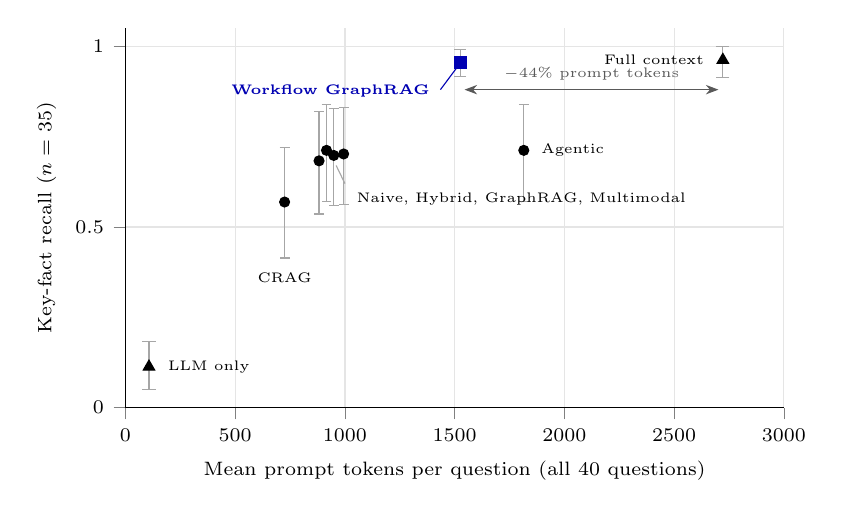
\begin{tikzpicture}
\begin{axis}[
  width=0.82\textwidth, height=6.4cm,
  xmin=0, xmax=3000, ymin=0, ymax=1.05,
  xlabel={Mean prompt tokens per question (all 40 questions)},
  ylabel={Key-fact recall ($n=35$)},
  xlabel style={font=\scriptsize}, ylabel style={font=\scriptsize},
  ticklabel style={font=\scriptsize},
  scaled x ticks=false, xtick={0,500,...,3000}, xticklabel style={/pgf/number format/1000 sep={}},
  axis lines*=left, tick align=outside, clip=false,
  grid=major, grid style={gray!20},
  error bars/error bar style={gray!70},
]
% chunk-retrieval baselines
\addplot[black, only marks, mark=*, mark size=1.8pt, error bars/.cd, y dir=both, y explicit]
coordinates {
 (916,0.712)  += (0,0.128) -= (0,0.141)
 (882,0.683)  += (0,0.136) -= (0,0.147)
 (949,0.698)  += (0,0.131) -= (0,0.138)
 (994,0.702)  += (0,0.129) -= (0,0.140)
 (1815,0.712) += (0,0.128) -= (0,0.141)
 (725,0.569)  += (0,0.150) -= (0,0.155)
};
% reference systems
\addplot[black, only marks, mark=triangle*, mark size=2.4pt, error bars/.cd, y dir=both, y explicit]
coordinates {
 (107,0.113)  += (0,0.070) -= (0,0.063)
 (2722,0.962) += (0,0.038) -= (0,0.048)
};
% proposed
\addplot[blue!70!black, only marks, mark=square*, mark size=2.2pt, error bars/.cd, y dir=both, y explicit]
coordinates {(1525,0.955) += (0,0.035) -= (0,0.038)};
\ifshoworacle
\addplot[blue!70!black, only marks, mark=square, mark size=2.2pt, error bars/.cd, y dir=both, y explicit]
coordinates {(1479,0.962) += (0,0.038) -= (0,0.048)};
\node[font=\tiny, anchor=east, blue!70!black] at (axis cs:1440,1.01) {Selection-Matched};
\fi
% labels
\node[font=\tiny, anchor=north west] at (axis cs:1010,0.62) {Naive, Hybrid, GraphRAG, Multimodal};
\draw[gray!70, thin] (axis cs:1000,0.62) -- (axis cs:960,0.67);
\node[font=\tiny, anchor=north] at (axis cs:725,0.40) {CRAG};
\node[font=\tiny, anchor=west] at (axis cs:1850,0.712) {Agentic};
\node[font=\tiny, anchor=west] at (axis cs:150,0.113) {LLM only};
\node[font=\tiny, anchor=east, blue!70!black] at (axis cs:1430,0.875) {\textbf{Workflow GraphRAG}};
\draw[blue!70!black, thin] (axis cs:1435,0.88) -- (axis cs:1515,0.945);
\node[font=\tiny, anchor=east] at (axis cs:2680,0.962) {Full context};
\draw[{Stealth[length=1.6mm]}-{Stealth[length=1.6mm]}, gray!70!black] (axis cs:1545,0.88) -- node[above, font=\tiny]{$-44\%$ prompt tokens} (axis cs:2702,0.88);
\end{axis}
\end{tikzpicture}
\caption{Key-fact recall against mean prompt tokens for all evaluated systems. Error bars show 95\% bootstrap confidence intervals. Circles: chunk-retrieval baselines; triangles: reference systems; squares: systems using rule-based SOP selection. Workflow GraphRAG reaches recall numerically close to full-context prompting with 44\% fewer prompt tokens.}
\label{fig:tradeoff}
\end{figure}

\begin{table}[!htbp]
\centering
\caption{Operational resource consumption per query across evaluated systems: mean prompt and completion tokens, mean generator invocations, and median execution latency across all 40 questions.}
\label{tab:cost}
\small
\setlength{\tabcolsep}{4pt}
\resizebox{\textwidth}{!}{%
\begin{tabular}{lcccc}
\toprule
System & Prompt tok. & Completion tok. & LLM calls & Latency (s) \\
\midrule
Naive RAG & 916 & 555 & 0.75 & 9.9 \\
GraphRAG (entity) & 949 & 559 & 0.75 & 9.6 \\
\textbf{Workflow GraphRAG} & 1525 & 710 & 0.95 & 10.7 \\
Hybrid RAG & 882 & 566 & 0.75 & 9.3 \\
Agentic RAG & 1815 & 1857 & 3.27 & 28.7 \\
Corrective RAG & 725 & 661 & 1.05 & 12.7 \\
Multimodal-layout RAG & 994 & 561 & 0.75 & 9.8 \\
LLM only & 107 & 792 & 1.00 & 10.4 \\
Full context & 2722 & 792 & 1.00 & 12.1 \\
\bottomrule
\end{tabular}
}
\end{table}

The mean number of generator invocations per query reflects deterministic refusal logic: Naive RAG and chunk-based baselines refuse queries with cosine similarity below $\tau = 0.3$ without invoking the generator (evaluating 30 of 40 queries, yielding a mean of $30/40 = 0.75$ calls per query). Workflow GraphRAG executes deterministic refusal only when no SOP score reaches 3 and vector similarity is below 0.3 (refusing 2 of 40 queries prior to inference, yielding $38/40 = 0.95$ calls per query). Full-context prompting evaluates all 40 queries directly ($40/40 = 1.00$ calls). In contrast, Agentic RAG invokes the generator iteratively within its ReAct search loop, averaging 3.27 calls per query.

Execution latency remains practical: Workflow GraphRAG exhibits a median latency of 10.7 seconds on local hardware, comparable to Naive RAG (9.9~s) and Full-Context Prompting (12.1~s). In contrast, Agentic RAG requires multiple ReAct iterations, resulting in 1,815 prompt tokens, 1,857 completion tokens, and a median latency of 28.7 seconds without improving factual accuracy (0.712 KFR).

We distinguish prompt-token savings from total operational expenditures: local deployment eliminates per-token API charges, but requires dedicated hardware memory and compute resources, which were not financially measured.

\subsection{Embedding sensitivity ablation}
\label{sec:ablation-embedding}
To examine retrieval sensitivity, we repeated evaluations of Naive RAG, GraphRAG, and Workflow GraphRAG using the non-fine-tuned base embedding model (\texttt{all-indo-e5-small-v4} base) instead of the fine-tuned checkpoint (Table~\ref{tab:ablation}).

\begin{table}[!htbp]
\centering
\caption{Ablation evaluating fine-tuned (v3) versus non-fine-tuned base embedding representations: key-fact recall and step coverage across primary systems.}
\label{tab:ablation}
\small
\begin{tabular}{lcc}
\toprule
System & v3 embedding & Base embedding \\
\midrule
Naive RAG & 0.712 / 0.727 & 0.910 / 0.898 \\
GraphRAG (entity) & 0.698 / 0.687 & 0.900 / 0.865 \\
\textbf{Workflow GraphRAG} & 0.955 / 1.000 & 0.955 / 1.000 \\
\bottomrule
\end{tabular}

\end{table}

Under the base embedding model, Naive RAG performance increases substantially from 0.712 to 0.910 KFR (and step coverage from 0.727 to 0.898). Similarly, custom entity-graph GraphRAG increases from 0.698 to 0.900 KFR. Workflow GraphRAG remains consistent at 0.955 KFR.
Figure~\ref{fig:embedding} visualises this shift.

\begin{figure}[!htbp]
\centering
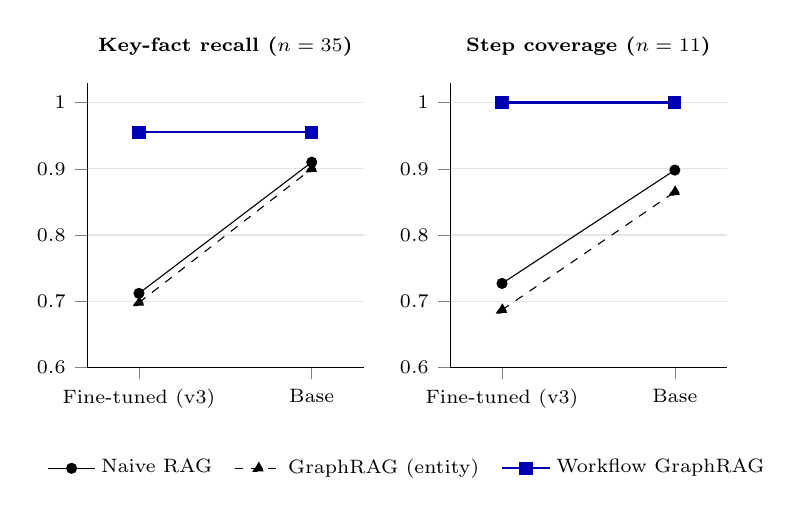
\begin{tikzpicture}
\pgfplotsset{abl/.style={
  width=0.42\textwidth, height=5.2cm,
  xmin=-0.3, xmax=1.3, ymin=0.6, ymax=1.03,
  xtick={0,1}, xticklabels={Fine-tuned (v3), Base},
  ticklabel style={font=\scriptsize}, title style={font=\scriptsize\bfseries},
  axis lines*=left, tick align=outside, ymajorgrids, grid style={gray!20},
  yticklabel style={/pgf/number format/fixed, /pgf/number format/precision=2}}}
\begin{axis}[abl, name=kfr, title={Key-fact recall ($n=35$)}]
\addplot[black, mark=*, mark size=1.8pt] coordinates {(0,0.712) (1,0.910)};
\addplot[black, dashed, mark=triangle*, mark size=2.2pt] coordinates {(0,0.698) (1,0.900)};
\addplot[blue!70!black, thick, mark=square*, mark size=2pt] coordinates {(0,0.955) (1,0.955)};
\end{axis}
\begin{axis}[abl, at={(kfr.east)}, anchor=west, xshift=1.1cm, title={Step coverage ($n=11$)},
  legend style={font=\scriptsize, draw=none, at={(-0.15,-0.28)}, anchor=north, legend columns=3, /tikz/every even column/.append style={column sep=6pt}}]
\addplot[black, mark=*, mark size=1.8pt] coordinates {(0,0.727) (1,0.898)};
\addplot[black, dashed, mark=triangle*, mark size=2.2pt] coordinates {(0,0.687) (1,0.865)};
\addplot[blue!70!black, thick, mark=square*, mark size=2pt] coordinates {(0,1.000) (1,1.000)};
\legend{Naive RAG, GraphRAG (entity), Workflow GraphRAG}
\end{axis}
\end{tikzpicture}
\caption{Embedding sensitivity: key-fact recall and step coverage with the fine-tuned (v3) and the non-fine-tuned base \texttt{all-indo-e5-small-v4} embedding. Chunk-retrieval baselines improve markedly with the base model, whereas Workflow GraphRAG is unchanged.}
\label{fig:embedding}
\end{figure}

This reveals substantial sensitivity to embedding configuration. Replacing the fine-tuned checkpoint with its base counterpart substantially improved the retrieval and recall performance of conventional chunk-based baselines, while Workflow GraphRAG remained consistent at 0.955 KFR. Although overfitting to the phrasing of the 50 fine-tuning question-answer pairs is a plausible hypothesis, the present experiments do not establish the definitive mechanism behind this degradation. Alternative factors include objective mismatch between contrastive loss and administrative chunk retrieval, training instability on small sample volumes, or distortions in embedding-space geometry. Regardless of the underlying cause, this comparison demonstrates that well-configured standard retrieval baselines perform competitively on this corpus (0.910 KFR), substantially narrowing the performance margin between conventional chunk retrieval and workflow-guided methods.

\subsection{Qualitative error analysis}
Analysis of generated outputs reveals specific behavioral differences across architectures:
\begin{enumerate}[leftmargin=*]
\item \textbf{Cross-SOP Disambiguation (Question X-2):} For inquiry ``Who signs the academic leave permit and late tuition permit letters, respectively?'', Naive RAG retrieved chunks from both procedures but failed to map officials to specific documents, listing multiple candidate signatories under each heading (KFR = 0.5). Workflow GraphRAG leveraged explicit step output attributes to assign signatories unambiguously (``Dean for Academic Leave Permit; Vice Dean for Resources for Late Tuition Permit''), achieving KFR = 1.0.
\item \textbf{Omission of Conditional Qualifications (Question IRS-A1):} In course registration inquiry ``Who approves the IRS form and how?'', the official procedure specifies that the academic advisor approves online via SIAP once credit loads are verified. Workflow GraphRAG correctly identified the advisor and SIAP portal, but omitted the prerequisite credit-load condition, scoring KFR = 0.667.
\item \textbf{Formatting Artifacts in Step Scoring (Question UKT-P1):} In late tuition payment, the selection-matched text ablation outputted step actors and actions on separate markdown lines. While complete and correct upon human inspection, the line-segmented automatic scorer registered partial step detection, illustrating measurement sensitivity to generator output formatting.
\end{enumerate}

%% ===================================================================
\section{Discussion and threats to validity}
\label{sec:discussion}

\subsection{Empirical findings and architectural interpretation}
The empirical results establish two distinct conclusions:
\begin{enumerate}[leftmargin=*]
\item \textbf{Demonstrated Finding:} The complete Workflow GraphRAG system, combining rule-based procedure selection and structured workflow blocks, achieves high factual completeness (0.955 KFR) and step coverage (1.000) on the institutional benchmark, attaining factual recall numerically close to full-context prompting while utilizing 44\% fewer prompt tokens.
\item \textbf{Non-Demonstrated Finding:} Explicit graph-derived workflow serialization was \emph{not} demonstrated to provide a statistically detectable factual accuracy advantage over providing the selected procedure's raw text ($p = 0.59$).
\end{enumerate}

This indicates that in concise, linear administrative workflows, procedure-level selection is an essential differentiator compared to unconstrained passage retrieval. When standard top-$k$ retrieval injects three competing procedures into the prompt, the small model suffers procedural cross-contamination. Resolving procedure selection---whether via rule-based routing, metadata filtering, or workflow indexing---mitigates this failure mode. However, the current experimental design does not fully isolate selection's causal contribution from accompanying query-expansion and context-budgeting variations. The empirical value of explicit graph structuring in this setting lies in standardized output formatting, concise prompt presentation, and explicit deliverable attribution, rather than an incremental gain in factual recall.

\subsection{Threats to internal and comparative validity}
We transparently identify key threats to validity:
\begin{itemize}[leftmargin=*]
\item \textbf{Custom Baseline Implementation:} The entity-graph GraphRAG baseline was constructed by the authors using 17 hand-curated relational triples. It does not represent published, automated frameworks such as Microsoft GraphRAG \cite{edge2024graphrag} or LightRAG \cite{guo2024lightrag}. While the observed comparison ($p=0.034$) is valid against this custom baseline, it should not be construed as a generalized claim against the GraphRAG paradigm.
\item \textbf{Author Benchmark Curation and Verification:} Benchmark questions, reference answers, and gold step annotations were developed and verified by the first author against official PDFs. Although verified against source documents, verification was not conducted by an independent administrative panel, introducing potential alignment between benchmark design and evaluated capabilities.
\item \textbf{Sample Size and Multiplicity Constraints:} The benchmark comprises 40 verified questions. The comparison between Workflow GraphRAG and Naive RAG yielded a borderline adjusted result ($p = 0.053$). While bootstrap confidence intervals suggest positive separation, statistical power is constrained at $n=40$.
\item \textbf{Scope of Scorer Audit:} The manual scorer audit validated 60 sampled rows across three systems, confirming 0.983 agreement and zero actor errors in that sample. This audit establishes scorer reliability, but cannot be extrapolated to assert zero actor errors across all uninspected outputs.
\end{itemize}

\subsection{Corpus and generalizability limitations}
\begin{itemize}[leftmargin=*]
\item \textbf{Linear, Short Procedures:} The corpus comprises 7 one-page linear procedures totaling 1,097 words. These workflows contain no conditional branching, parallel executions, or decision gateways. While representative of institutional student services, findings cannot be generalized directly to complex, branching enterprise workflows where formal BPMN gateways may prove essential.
\item \textbf{Rule-Based Selection Transferability:} The selection mechanism utilizes keyword and alias heuristics tailored to this 7-SOP collection. In large-scale corpora containing hundreds of procedures, manual alias curation is impractical; automated classification or hierarchical vector routing would be required.
\item \textbf{Supporting Chunk Contamination:} Appending top-3 vector chunks after the workflow block reintroduces passages from unselected SOPs. Future ablations should isolate the impact of removing or filtering supporting chunks to strictly within-SOP passages.
\item \textbf{Single Generator Architecture:} Evaluations were conducted on a single local small model (\texttt{gemma4:e2b}) at temperature 0. Evaluating across additional model families (e.g., Llama-3.2, Qwen-2.5) is necessary to determine model invariance.
\end{itemize}

%% ===================================================================
\section{Conclusion and future work}
\label{sec:conclusion}

This study investigated the empirical relationship between Standard Operating Procedure selection and explicit workflow graph structuring in local retrieval-augmented question answering. Evaluating across 10 system configurations on 40 verified institutional questions using a locally hosted small generator (\texttt{gemma4:e2b}), we addressed our core research questions:
\begin{itemize}[leftmargin=*]
\item \textbf{RQ1 (Answer Quality):} Workflow GraphRAG achieved 0.955 key-fact recall and 1.000 step coverage, improving upon naive chunk retrieval (0.712 KFR, Holm $p=0.053$) and custom entity-graph retrieval (0.698 KFR, Holm $p=0.034$). In step order preservation, Workflow GraphRAG achieved an observed TIR of 0.000, whereas custom entity-graph RAG and full-context prompting exhibited non-zero inversion rates of 0.083 and 0.027.
\item \textbf{RQ2 (Selection vs.\ Structuring):} A controlled selection-matched text ablation achieved 0.962 KFR. A paired Wilcoxon test detected no statistically significant difference between graph-structured context and selected raw text ($p=0.59$), confirming that explicit graph serialization yielded no incremental factual recall benefit over providing the selected procedure's raw text on this benchmark.
\item \textbf{RQ3 (Refusal):} The system achieved 1.000 refusal accuracy on 5 unanswerable questions through a combination of selection-threshold filtering and generated refusals.
\item \textbf{RQ4 (Efficiency):} Workflow GraphRAG consumed 1,525 prompt tokens per query, attaining factual recall numerically close to full-context prompting while reducing prompt tokens by 44\%.
\end{itemize}

For institutional practitioners deploying small language models over concise procedural documents, our findings emphasize the practical value of procedure-level selection for reducing cross-document distractor interference. Explicit workflow graphs provide structured output consistency, guarantee chronological ordering, and reduce prompt tokens relative to full context, but do not automatically increase factual recall over well-selected raw text.

Future work will focus on: (1) replacing heuristic rule selection with learned dense procedural classifiers; (2) scaling workflow representations to branching procedures by parsing official BPMN XML diagrams; (3) evaluating against published open-source GraphRAG implementations (LightRAG, HippoRAG); and (4) conducting an a priori powered evaluation with independent administrative validation.

\section*{Acknowledgements}
This research did not receive any specific grant from funding agencies in the public, commercial, or not-for-profit sectors. The authors thank the Dean of the Faculty of Science and Mathematics, Universitas Diponegoro, Prof.\ Dr.\ Kusworo Adi, the Head of the Department of Informatics, Dr.\ Aris Sugiharto, the Undergraduate Thesis Coordinator, Nurdin Bahtiar, and the thesis examiners, Dr.\ Sutikno and Yunila Dwi Putri Ariyanti, for their guidance and feedback, and the Faculty of Science and Mathematics for permitting this research to be carried out using its SOPs.

\section*{Data and code availability}
Code, benchmark, and evaluation scripts are available at \url{https://github.com/reon01425-glitch/Chatbot-RAG-Comparison}, branch \url{exp/full-run-v1}. Experimental logs are deposited in \url{results/full_v3_20261008/} (main run) and \url{results/full_base_20261008/} (embedding ablation). The repository includes the 7 source SOP documents redistributed under institutional permission.

\section*{CRediT authorship contribution statement}
\textbf{Cipta Fikri Wiratama}: Conceptualization, Methodology, Software, Data curation, Validation, Investigation, Writing -- original draft. \textbf{Indra Waspada}: Conceptualization, Supervision, Writing -- review \& editing. \textbf{Dhena Kamalia Fu'adi}: Data curation, Validation, Writing -- review \& editing. \textbf{Ramona Ramli}: Conceptualization, Methodology, Supervision, Writing -- review \& editing. \textbf{Henri Tantyoko}: Methodology, Validation, Writing -- review \& editing. \textbf{Sandy Kurniawan}: Supervision, Methodology, Writing -- review \& editing. \textbf{Satriawan Rasyid Purnama}: Validation, Formal analysis, Writing -- review \& editing.

\section*{Declaration of competing interest}
The authors declare no competing interests.

\section*{Declaration of generative AI use}
During the preparation of this work, the authors used generative AI tools to assist with productivity in literature search, drafting, and academic language editing. All methodological formulations, system implementations, and experimental analyses were designed by the authors, who reviewed and edited all generated text and assume full responsibility for the published content.

\appendix
\section{Full results with confidence intervals}
\label{app:full-results}
Table~\ref{tab:results-full} presents the complete evaluation results across all 10 systems, reporting mean values alongside 95\% bootstrap confidence intervals (10,000 resamples).

\begin{table}[!htbp]
\centering
\caption{Complete evaluation results across all 10 systems on \nVerified{} verified benchmark questions, reporting mean [95\% bootstrap confidence intervals].}
\label{tab:results-full}
\scriptsize
\setlength{\tabcolsep}{2pt}
\resizebox{\textwidth}{!}{%
\begin{tabular}{lccccccc}
\toprule
System & KFR $\uparrow$ & Coverage $\uparrow$ & TIR $\downarrow$ & AMR $\downarrow$ & Refusal acc. $\uparrow$ & False ref. $\downarrow$ & Prompt tok. \\
\midrule
Naive RAG & 0.712 [0.571, 0.840] & 0.727 [0.455, 1.000] & 0.000 [0.000, 0.000] & 0.000 [0.000, 0.000] & 0.600 [0.200, 1.000] & 0.000 [0.000, 0.000] & 916 \\
GraphRAG (entity) & 0.698 [0.560, 0.829] & 0.687 [0.415, 0.920] & 0.083 [0.000, 0.250] & 0.000 [0.000, 0.000] & 0.600 [0.200, 1.000] & 0.000 [0.000, 0.000] & 949 \\
\textbf{Workflow GraphRAG} & 0.955 [0.917, 0.990] & 1.000 [1.000, 1.000] & 0.000 [0.000, 0.000] & 0.000 [0.000, 0.000] & 1.000 [1.000, 1.000] & 0.000 [0.000, 0.000] & 1525 \\
\textit{Selection-Matched Text RAG (ablation)} & 0.962 [0.914, 1.000] & 0.975 [0.926, 1.000] & 0.000 [0.000, 0.000] & 0.000 [0.000, 0.000] & 1.000 [1.000, 1.000] & 0.000 [0.000, 0.000] & 1479 \\
\midrule
Hybrid RAG & 0.683 [0.536, 0.819] & 0.712 [0.439, 0.970] & 0.000 [0.000, 0.000] & 0.000 [0.000, 0.000] & 0.600 [0.200, 1.000] & 0.000 [0.000, 0.000] & 882 \\
Agentic RAG & 0.712 [0.571, 0.840] & 0.702 [0.430, 0.950] & 0.000 [0.000, 0.000] & 0.000 [0.000, 0.000] & 0.600 [0.200, 1.000] & 0.000 [0.000, 0.000] & 1815 \\
Corrective RAG & 0.569 [0.414, 0.719] & 0.636 [0.364, 0.909] & 0.000 [0.000, 0.000] & 0.000 [0.000, 0.000] & 1.000 [1.000, 1.000] & 0.371 [0.229, 0.543] & 725 \\
Multimodal-layout RAG & 0.702 [0.562, 0.831] & 0.702 [0.430, 0.950] & 0.000 [0.000, 0.000] & 0.000 [0.000, 0.000] & 0.600 [0.200, 1.000] & 0.000 [0.000, 0.000] & 994 \\
\midrule
LLM only & 0.113 [0.050, 0.183] & 0.105 [0.000, 0.209] & 0.333 [0.000, 0.667] & 0.444 [0.000, 1.000] & 0.000 [0.000, 0.000] & 0.000 [0.000, 0.000] & 107 \\
Full context & 0.962 [0.914, 1.000] & 0.944 [0.871, 1.000] & 0.027 [0.000, 0.082] & 0.000 [0.000, 0.000] & 1.000 [1.000, 1.000] & 0.000 [0.000, 0.000] & 2722 \\
\bottomrule
\end{tabular}
}
\end{table}

\section{Entity-graph baseline triples}
\label{app:triples}
Table~\ref{tab:triples} lists the 17 relational triples used by the custom entity-graph GraphRAG baseline.

\begin{table}[!htbp]
\centering
\caption{The 17 hand-curated relational triples of the custom entity-graph GraphRAG baseline, as defined in \texttt{src/engine.py}. Entities and relations are kept in their original Indonesian form.}
\label{tab:triples}
\scriptsize
\setlength{\tabcolsep}{4pt}
\begin{tabular}{rlll}
\toprule
\# & Head entity & Tail entity & Relation \\
\midrule
1 & cuti akademik & izin cuti & prosedur pengajuan \\
2 & cuti akademik & aktif kembali & alur lanjutan \\
3 & cuti akademik & ketua program studi & rekomendasi \& persetujuan \\
4 & cuti akademik & dekan & penerbitan SK izin \\
5 & cuti akademik & spp/ukt & syarat bebas tunggakan \\
6 & legalisir & ijazah & dokumen objek \\
7 & legalisir & transkrip & dokumen objek \\
8 & legalisir & subbagian akademik & verifikasi \& validasi \\
9 & beasiswa & rekomendasi beasiswa & dokumen pengajuan \\
10 & beasiswa & wakil dekan i & pengesahan surat \\
11 & ukt & keterlambatan pembayaran & permohonan dispensasi \\
12 & ukt & bagian keuangan fsm & verifikasi pembayaran \\
13 & irs & pengisian irs & registrasi akademik per semester \\
14 & irs & dosen wali & bimbingan \& persetujuan online \\
15 & irs & siap undip & portal sistem informasi \\
16 & organisasi mahasiswa & proposal kegiatan & pengajuan persetujuan \\
17 & organisasi mahasiswa & wakil dekan i & persetujuan kegiatan \\
\bottomrule
\end{tabular}
\end{table}

\section{Example benchmark questions}
\label{app:examples}
Table~\ref{tab:examples} gives one benchmark question per category.

\begin{table}[!htbp]
\centering
\caption{One benchmark question per category from \texttt{sop\_benchmark\_v1.json}, with English glosses.}
\label{tab:examples}
\scriptsize
\setlength{\tabcolsep}{3pt}
\begin{tabularx}{\textwidth}{l l >{\raggedright\arraybackslash}X}
\toprule
ID & Category & Question (Indonesian) / English gloss \\
\midrule
CUTI-P1 & Procedural & \textit{Apa saja tahapan mengajukan cuti akademik di FSM dari awal sampai surat izin keluar, dan siapa yang mengerjakan tiap tahap?} \newline What are the steps for applying for academic leave at FSM, from the start until the permit letter is issued, and who performs each step? \\
CUTI-A1 & Actor & \textit{Setelah form cuti saya ditandatangani Kaprodi, form itu diserahkan ke siapa dan diproses oleh bagian apa?} \newline After the Head of Study Programme signs my leave form, to whom is it submitted and which unit processes it? \\
CUTI-D1 & Documents & \textit{Dokumen apa saja yang harus dilampirkan saat mengajukan cuti akademik?} \newline Which documents must be attached when applying for academic leave? \\
CUTI-T1 & Time/location & \textit{Berapa lama maksimal proses izin cuti akademik, dan di mana saya mengambil Surat Izin Dekan?} \newline What is the maximum processing time for an academic leave permit, and where do I collect the Dean's permit letter? \\
X-1 & Cross-SOP & \textit{Apa perbedaan dokumen yang dibawa untuk mengajukan cuti akademik dengan untuk aktif kembali setelah cuti?} \newline How do the documents required for academic leave differ from those required for reactivation after leave? \\
NA-1 & Unanswerable & \textit{Berapa biaya legalisir ijazah per lembar di FSM?} \newline How much does diploma legalisation cost per sheet at FSM? \\
\bottomrule
\end{tabularx}
\end{table}

%% ===================================================================
\small
\setlength{\bibsep}{2pt}
\begin{thebibliography}{99}

\bibitem{lewis2020rag}
P.~Lewis, E.~Perez, A.~Piktus, F.~Petroni, V.~Karpukhin, N.~Goyal, H.~K{\"u}ttler, M.~Lewis, W.~Yih, T.~Rockt{\"a}schel, S.~Riedel, D.~Kiela, Retrieval-augmented generation for knowledge-intensive {NLP} tasks, in: Advances in Neural Information Processing Systems 33 (NeurIPS 2020), 2020, pp. 9459--9474.

\bibitem{gao2023ragsurvey}
Y.~Gao, Y.~Xiong, X.~Gao, K.~Jia, J.~Pan, Y.~Bi, Y.~Dai, J.~Sun, M.~Wang, H.~Wang, Retrieval-augmented generation for large language models: A survey, arXiv:2312.10997 (2023).

\bibitem{edge2024graphrag}
D.~Edge, H.~Trinh, N.~Cheng, J.~Bradley, A.~Chao, A.~Mody, S.~Truitt, J.~Larson, From local to global: A graph {RAG} approach to query-focused summarization, arXiv:2404.16130 (2024).

\bibitem{peng2024graphragsurvey}
B.~Peng, Y.~Zhu, Y.~Liu, X.~Bo, H.~Shi, C.~Hong, Y.~Zhang, S.~Tang, Graph retrieval-augmented generation: A survey, arXiv:2408.08921 (2024).

\bibitem{robertson2009bm25}
S.~Robertson, H.~Zaragoza, The probabilistic relevance framework: {BM25} and beyond, Foundations and Trends in Information Retrieval 3~(4) (2009) 333--389.

\bibitem{cormack2009rrf}
G.~V. Cormack, C.~L.~A. Clarke, S.~B{\"u}ttcher, Reciprocal rank fusion outperforms {C}ondorcet and individual rank learning methods, in: Proceedings of the 32nd International ACM SIGIR Conference on Research and Development in Information Retrieval, 2009, pp. 758--759.

\bibitem{yao2023react}
S.~Yao, J.~Zhao, D.~Yu, N.~Du, I.~Shafran, K.~Narasimhan, Y.~Cao, {ReAct}: Synergizing reasoning and acting in language models, in: International Conference on Learning Representations (ICLR), 2023.

\bibitem{yan2024crag}
S.-Q. Yan, J.-C. Gu, Y.~Zhu, Z.-H. Ling, Corrective retrieval augmented generation, arXiv:2401.15884 (2024).

\bibitem{asai2024selfrag}
A.~Asai, Z.~Wu, Y.~Wang, A.~Sil, H.~Hajishirzi, {Self-RAG}: Learning to retrieve, generate, and critique through self-reflection, in: International Conference on Learning Representations (ICLR), 2024.

\bibitem{liu2024lost}
N.~F. Liu, K.~Lin, J.~Hewitt, A.~Paranjape, M.~Bevilacqua, F.~Petroni, P.~Liang, Lost in the middle: How language models use long contexts, Transactions of the Association for Computational Linguistics 12 (2024) 157--173.

\bibitem{pan2024unifying}
S.~Pan, L.~Luo, Y.~Wang, C.~Chen, J.~Wang, X.~Wu, Unifying large language models and knowledge graphs: A roadmap, IEEE Transactions on Knowledge and Data Engineering 36~(7) (2024) 3580--3599.

\bibitem{guo2024lightrag}
Z.~Guo, L.~Xia, Y.~Yu, T.~Ao, C.~Huang, {LightRAG}: Simple and fast retrieval-augmented generation, arXiv:2410.05779 (2024).

\bibitem{gutierrez2024hipporag}
B.~J. Guti{\'e}rrez, Y.~Shu, Y.~Gu, M.~Yasunaga, Y.~Su, {HippoRAG}: Neurobiologically inspired long-term memory for large language models, in: Advances in Neural Information Processing Systems 37 (NeurIPS 2024), 2024.

\bibitem{lin2026sedrag}
L.~Lin, Z.~Zhu, T.~Zhang, Y.~Wen, {SOPRAG}: Multi-view graph experts retrieval for industrial standard operating procedures, arXiv:2602.01858 (2026).

\bibitem{wu2026okhrag}
K.~Wu, C.~Kuai, Z.~Li, J.~Jiang, S.~Shen, S.~Wang, C.-W.~Hu, Z.~Tu, Y.~Zhou, Knowledge is not static: Order-aware hypergraph {RAG} for language models, arXiv:2604.12185 (2026).

\bibitem{dumas2018fundamentals}
M.~Dumas, M.~La~Rosa, J.~Mendling, H.~A. Reijers, Fundamentals of Business Process Management, 2nd Edition, Springer, 2018.

\bibitem{omg2011bpmn}
Object Management Group, Business Process Model and Notation ({BPMN}), Version 2.0, OMG Standard formal/2011-01-03 (2011). Also published as ISO/IEC 19510:2013.

\bibitem{friedrich2011process}
F.~Friedrich, J.~Mendling, F.~Puhlmann, Process model generation from natural language text, in: Advanced Information Systems Engineering (CAiSE 2011), Vol. 6741 of Lecture Notes in Computer Science, Springer, 2011, pp. 482--496.

\bibitem{lazarusnlp_e5}
LazarusNLP, all-indo-e5-small-v4, Hugging Face model card, \url{https://huggingface.co/LazarusNLP/all-indo-e5-small-v4}, accessed May 2026.

\bibitem{wang2022e5}
L.~Wang, N.~Yang, X.~Huang, B.~Jiao, L.~Yang, D.~Jiang, R.~Majumder, F.~Wei, Text embeddings by weakly-supervised contrastive pre-training, arXiv:2212.03533 (2022).

\bibitem{henderson2017mnr}
M.~Henderson, R.~Al-Rfou, B.~Strope, Y.-H. Sung, L.~Luk{\'a}cs, R.~Guo, S.~Kumar, B.~Miklos, R.~Kurzweil, Efficient natural language response suggestion for smart reply, arXiv:1705.00652 (2017).

\bibitem{lin2004rouge}
C.-Y. Lin, {ROUGE}: A package for automatic evaluation of summaries, in: Text Summarization Branches Out, Association for Computational Linguistics, 2004, pp. 74--81.

\bibitem{es2024ragas}
S.~Es, J.~James, L.~Espinosa-Anke, S.~Schockaert, {RAGAs}: Automated evaluation of retrieval augmented generation, in: Proceedings of the 18th Conference of the European Chapter of the Association for Computational Linguistics: System Demonstrations, 2024, pp. 150--158.

\bibitem{zheng2023judging}
L.~Zheng, W.-L. Chiang, Y.~Sheng, S.~Zhuang, Z.~Wu, Y.~Zhuang, Z.~Lin, Z.~Li, D.~Li, E.~P. Xing, H.~Zhang, J.~E. Gonzalez, I.~Stoica, Judging {LLM}-as-a-judge with {MT-Bench} and {Chatbot Arena}, in: Advances in Neural Information Processing Systems 36 (NeurIPS 2023), Datasets and Benchmarks Track, 2023.

\bibitem{efron1993bootstrap}
B.~Efron, R.~J. Tibshirani, An Introduction to the Bootstrap, Chapman \& Hall/CRC, 1993.

\bibitem{wilcoxon1945}
F.~Wilcoxon, Individual comparisons by ranking methods, Biometrics Bulletin 1~(6) (1945) 80--83.

\bibitem{holm1979}
S.~Holm, A simple sequentially rejective multiple test procedure, Scandinavian Journal of Statistics 6~(2) (1979) 65--70.

\end{thebibliography}

\end{document}
